%===============================================================================
\chapter{The Renormalization Group as Algebra and Geometry}
\label{ch:rg_geometry}
%===============================================================================

\marginnote{The Prologue showed \emph{that} parameters run. This chapter develops the \textbf{complete framework}: the Callan-Symanzik equation has a unified algebraic-geometric structure. Algebra and geometry are not alternatives---they are two faces of the same coin, emerging together from the equation. This framework is exact and independent of any computational method.}

%===============================================================================
% PART I: THE PHYSICAL FOUNDATION
%===============================================================================

%-------------------------------------------------------------------------------
\section{From Running Parameters to Structure}
\label{sec:running_to_structure}
%-------------------------------------------------------------------------------

The Prologue ended with a remarkable result. For the damped anharmonic oscillator, demanding the cancellation of secular terms forced the amplitude and phase to satisfy:
\begin{align}
\frac{dA}{dt} &= -\gamma A \label{eq:recap_A}\\
\frac{d\phi}{dt} &= \frac{3\epsilon A^2}{8\omega_0} \label{eq:recap_phi}
\end{align}
The amplitude $A$ decays exponentially due to damping, while the phase $\phi$ advances at a rate proportional to $\epsilon A^2$. These are the \textbf{RG equations} for the oscillator---but three questions immediately arise:

\begin{center}
\fbox{\parbox{0.85\textwidth}{
\textbf{Question 1:} Where do the parameters $(A, \phi)$ ``live''?\\[4pt]
\textbf{Question 2:} What mathematical structure governs their evolution?\\[4pt]
\textbf{Question 3:} Why does the same structure appear in statistical mechanics, QFT, and PDEs?
}}
\end{center}

The answers reveal that the renormalization group is not merely a collection of techniques---it has deep mathematical structure. \textbf{Crucially, this structure is simultaneously algebraic and geometric}:

\begin{center}
\fbox{\parbox{0.85\textwidth}{
\textbf{The central insight of this chapter:} Algebra and geometry are not alternative ways of viewing RG. They are \emph{two faces of the same structure}, emerging together from the Callan-Symanzik equation.
}}
\end{center}

\begin{itemize}
\item Scale transformations form a \textbf{Lie group}---this is algebraic
\item The group acts on a \textbf{manifold} (theory space)---this is geometric
\item The beta function is both the \textbf{Lie algebra generator} and a \textbf{vector field}---the same object in two languages
\item Scheme transformations are both \textbf{group elements} and \textbf{diffeomorphisms}---again, two names for one thing
\end{itemize}

Table~\ref{tab:correspondence} is not a dictionary between separate subjects; it shows that each RG concept is intrinsically both algebraic and geometric. This chapter develops each row, showing how they emerge organically from the central equation.

\begin{table}[h!]
\centering
\renewcommand{\arraystretch}{1.4}
\caption{The correspondence between Lie theory and the renormalization group.}
\label{tab:correspondence}
\begin{tabular}{@{}ll@{}}
\toprule
\textbf{Algebraic/Geometric Concept} & \textbf{RG Interpretation} \\
\midrule
Dilation group $(\mathbb{R}^+, \times)$ & Scale transformations \\
Lie algebra generator $\mathcal{D}$ & Infinitesimal RG transformation \\
Vector field $\boldsymbol{\beta}$ on $\mathcal{M}$ & Beta functions \\
Integral curves of $\boldsymbol{\beta}$ & RG trajectories (flows) \\
Fixed points ($\boldsymbol{\beta} = 0$) & Scale-invariant theories \\
Lie derivative $L_{\boldsymbol{\beta}}$ & RG equation \\
Scaling dimension $\Delta$ & Eigenvalue of $\mathcal{D}$ \\
Connection $\Gamma^a_{bc}$ & Anomalous dimension matrix / OPE coefficients \\
Curvature $R^a{}_{bcd}$ & Scheme-independent invariants \\
\bottomrule
\end{tabular}
\end{table}

%-------------------------------------------------------------------------------
\section{Scale Independence: The Physical Foundation}
\label{sec:scale_independence}
%-------------------------------------------------------------------------------

\marginnote{The fundamental insight: physical predictions cannot depend on arbitrary choices of scale. This requirement \emph{determines} the beta functions.}

Why do parameters run? The answer is a beautiful consistency requirement: \textbf{physical predictions cannot depend on arbitrary choices of scale}. If we describe a system at scale $\mu_1$ or $\mu_2$, we must get the same physical answers. This seemingly innocuous statement has profound consequences.

\subsection{The Setup}

Consider a physical observable $\mathcal{O}$ that depends on:
\begin{itemize}
\item \textbf{External scales}: momenta $p$, energies $E$, positions $x$, times $t$
\item \textbf{Internal parameters}: couplings $g$, masses $m$
\item \textbf{Reference scale}: $\mu$ (the ``renormalization scale'')
\end{itemize}

The observable has \textbf{explicit} $\mu$-dependence from having chosen $\mu$ as our reference, and \textbf{implicit} $\mu$-dependence through the running parameters $g(\mu)$.

\subsection{The Callan-Symanzik Equation}

Physical predictions cannot depend on our arbitrary choice of $\mu$. Mathematically:
\begin{equation}
\mu\frac{d\mathcal{O}}{d\mu} = 0
\label{eq:scale_independence}
\end{equation}

But $\mathcal{O}$ depends on $\mu$ both explicitly and through the running couplings:
\begin{equation}
\mu\frac{d\mathcal{O}}{d\mu} = \mu\frac{\partial\mathcal{O}}{\partial\mu}\bigg|_g + \mu\frac{\partial g^i}{\partial\mu}\frac{\partial\mathcal{O}}{\partial g^i}
\end{equation}

Define the \textbf{beta functions}:
\begin{equation}
\beta^i(g) \equiv \mu\frac{\partial g^i}{\partial\mu}
\end{equation}

\marginnote{The beta function $\beta^i = \mu\,\partial g^i/\partial\mu$ tells us how parameters change when we change the reference scale.}

Then scale independence becomes:
\begin{equation}
\boxed{\left(\mu\frac{\partial}{\partial\mu} + \beta^i(g)\frac{\partial}{\partial g^i}\right)\mathcal{O} = 0}
\label{eq:callan_symanzik_basic}
\end{equation}

This is the \textbf{Callan-Symanzik equation} in its simplest form.

\begin{workedbox}[Box 2.1: Deriving the CS Equation from First Principles]
\textbf{Goal:} Show step-by-step why scale independence forces parameters to run.

\textbf{Setup:} Consider a physical quantity $\mathcal{O}(p/\mu, g(\mu))$ where $p$ is an external momentum, $\mu$ is the renormalization scale, and $g$ is a coupling.

\textbf{Step 1: The physics doesn't know about $\mu$.}

$\mu$ is our arbitrary choice of reference scale (like choosing units). Therefore:
\begin{equation}
\frac{d\mathcal{O}}{d\mu} = 0 \quad \text{(total derivative)}
\end{equation}

\textbf{Step 2: Chain rule expansion.}

$\mathcal{O}$ depends on $\mu$ in two ways:
\begin{itemize}
\item \textbf{Explicitly}: through the ratio $p/\mu$
\item \textbf{Implicitly}: through $g(\mu)$
\end{itemize}

By the chain rule:
\begin{equation}
\frac{d\mathcal{O}}{d\mu} = \frac{\partial\mathcal{O}}{\partial\mu}\bigg|_g + \frac{\partial g}{\partial\mu}\frac{\partial\mathcal{O}}{\partial g}\bigg|_\mu = 0
\end{equation}

\textbf{Step 3: Multiply by $\mu$ for convenience.}

Define $\beta(g) \equiv \mu\frac{\partial g}{\partial\mu}$. Then:
\begin{equation}
\mu\frac{\partial\mathcal{O}}{\partial\mu}\bigg|_g + \beta(g)\frac{\partial\mathcal{O}}{\partial g}\bigg|_\mu = 0
\end{equation}

\textbf{Step 4: Physical interpretation.}

If $\beta \neq 0$, then $\frac{\partial\mathcal{O}}{\partial\mu} \neq 0$. The explicit $\mu$-dependence must be \textit{compensated} by implicit $\mu$-dependence through running couplings.

\tcblower
\textbf{The punchline:} Scale independence doesn't mean ``nothing changes.'' It means ``changes in the explicit scale are exactly compensated by changes in the couplings.'' The beta function quantifies this compensation.
\end{workedbox}

\subsection{The Full CS Equation with Anomalous Dimensions}

For an $n$-point correlation function, the CS equation takes a richer form:
\begin{equation}
\left(\mu\frac{\partial}{\partial\mu} + \beta_r\frac{\partial}{\partial r} + \beta_\lambda\frac{\partial}{\partial\lambda} + n\gamma\right)\tilde{G}_n = 0
\label{eq:cs_full}
\end{equation}

The new term $n\gamma$ is the \textbf{anomalous dimension}. Each field $\phi$ contributes a factor $\gamma$---this is the quantum/interaction correction to the classical scaling dimension. We will see its origin both algebraically (as a representation label) and geometrically (as a connection coefficient).

%-------------------------------------------------------------------------------
\subsection{Scale Covariance: A Universal Structure}
\label{sec:scale_covariance}
%-------------------------------------------------------------------------------

Although we have written the Callan-Symanzik equation in the language of QFT, its structure appears whenever we have a notion of scale and a family of models: multiple-scale analysis of ODEs, similarity solutions of PDEs, and coarse-grained descriptions of stochastic dynamics. The later examples (oscillator, amplitude equation, PME) are included precisely to show that this geometric structure is not peculiar to quantum field theories.

The generic \textbf{scale-covariance equation} takes the form:
\begin{equation}
\left(\mu\frac{\partial}{\partial\mu} + \beta^i(g)\frac{\partial}{\partial g^i} + \Gamma(g)\right)F(x; \mu, g) = 0
\label{eq:generalized_cs}
\end{equation}
where $\mu$ is a scale parameter (which could be a momentum scale, time, length, or cutoff), $g^i$ are the model parameters, $\beta^i(g)$ describes how parameters change with scale, $\Gamma(g)$ captures anomalous scaling, and $F$ is an observable or solution.

\marginnote{The CS equation~\eqref{eq:callan_symanzik_basic} is one instance of the general scale-covariance structure~\eqref{eq:generalized_cs}. The same mathematical form appears across physics.}

In different contexts, this structure specializes as follows:
\begin{itemize}
\item \textbf{QFT}: $\mu$ is the renormalization scale, $F$ is a Green's function, and~\eqref{eq:generalized_cs} becomes the Callan-Symanzik equation
\item \textbf{Anharmonic oscillator}: ``Scale'' is the arbitrary time origin $t_0$, and demanding $dx/dt_0 = 0$ yields the same structure
\item \textbf{Similarity solutions of PDEs}: ``Scale'' is time or length; self-similarity imposes~\eqref{eq:generalized_cs} on the similarity profile
\item \textbf{Statistical mechanics}: $\mu$ is the coarse-graining scale in Wilsonian RG
\end{itemize}

The Wilsonian coarse-graining picture provides the physical foundation for why parameters run: integrating out short-wavelength fluctuations modifies effective couplings. The CS equation~\eqref{eq:callan_symanzik_basic} provides the analytic structure we develop in this chapter. Part V demonstrates the universality of~\eqref{eq:generalized_cs} through explicit examples.

%-------------------------------------------------------------------------------
\subsection{Theory Space}
\label{sec:theory_space_intro}
%-------------------------------------------------------------------------------

The parameters $g^i$ appearing in~\eqref{eq:generalized_cs} are coordinates on \textbf{theory space} $\mathcal{M}$---the space of all theories (or models) under consideration. Each point in $\mathcal{M}$ represents a specific choice of couplings, and hence a specific theory.

\marginnote{We work with a finite-dimensional truncation of theory space. Full Wilsonian theory space is infinite-dimensional (the space of all local functionals).}

We treat $\mathcal{M}$ as a finite-dimensional smooth manifold for clarity. This is a truncation: in full generality, Wilsonian theory space is infinite-dimensional (the space of all local action functionals). The finite-dimensional case captures the essential geometry while avoiding functional-analytic complications.

The distinction between the \textbf{CS equation}~\eqref{eq:callan_symanzik_basic} and the \textbf{RG flow equation}:
\begin{equation}
\frac{dg^i}{d\ell} = \beta^i(g), \qquad \ell = \log(\mu/\mu_0)
\end{equation}
is important. The CS equation is a PDE for correlation functions (or observables) on the extended space $(\mu, g)$. The RG flow equation~\eqref{eq:rg_ode} is an ODE on theory space $\mathcal{M}$ alone, with $\ell$ as the evolution parameter. They encode the same physics but emphasize different aspects: the CS equation focuses on observables, while~\eqref{eq:rg_ode} focuses on the flow of couplings.

%===============================================================================
% PART II: THE SYMMETRY STRUCTURE OF THE RG EQUATION
%===============================================================================

\marginnote{Part II develops the symmetry structure \emph{of} the Callan-Symanzik equation~\eqref{eq:callan_symanzik_basic}. We do not introduce new objects---we discover what structure the equation \emph{already has}.}

The Callan-Symanzik equation~\eqref{eq:callan_symanzik_basic} is a first-order partial differential equation. Like any differential equation, it has a \textbf{symmetry structure}---transformations that leave it invariant. Understanding this structure is not an alternative to understanding the equation; it \emph{is} understanding the equation.

We will find two intertwined symmetries:
\begin{enumerate}
\item \textbf{Scale transformations}: The equation is invariant under $\mu \to \lambda\mu$, which forms a Lie group
\item \textbf{Scheme transformations}: The equation holds in any scheme, so reparameterizations $g^i \to g'^i(g)$ are symmetries
\end{enumerate}

These are not independent---they combine into a single geometric object, as we will see in Part~III.

%-------------------------------------------------------------------------------
\section{Scale Invariance as a Lie Group}
\label{sec:dilation_algebra}
%-------------------------------------------------------------------------------

\marginnote{The dilation group is the simplest non-trivial Lie group: one-dimensional, abelian, and connected. Its Lie algebra has a single generator $\mathcal{D}$.}

Return to the CS equation~\eqref{eq:callan_symanzik_basic}:
\begin{equation}
\left(\mu\frac{\partial}{\partial\mu} + \beta^i(g)\frac{\partial}{\partial g^i}\right)\mathcal{O} = 0
\tag{\ref{eq:callan_symanzik_basic}}
\end{equation}

This equation is \textbf{covariant under scale transformations}: the physics is unchanged under the \emph{combined} transformation $(\mu, g) \to (\lambda\mu, g'(\lambda))$ where the couplings flow according to the beta function. Sending $\mu \to \lambda\mu$ with fixed $g$ does \textit{not} preserve the equation unless $\beta = 0$ (i.e., at a fixed point). Scale transformations form the \textbf{dilation group}, and the beta function $\beta^i$ is precisely its \textbf{generator}.

\marginnote{Mathematically: the dilation group is a 1-parameter Lie group. Physically: the induced RG flow on theory space is a \textbf{semigroup}---coarse-graining is irreversible.}

An important distinction: scale transformations on spacetime form a genuine \textbf{Lie group} (with inverses). However, the induced RG flow on coupling space is only a \textbf{semigroup}---Wilson's coarse-graining integrates out degrees of freedom, and this information loss cannot be reversed. True scale \emph{invariance} of correlation functions holds only at fixed points where $\beta^i(g^*) = 0$.

\subsection{The Dilation Group}

The operator $\mu\frac{\partial}{\partial\mu}$ in~\eqref{eq:callan_symanzik_basic} generates scale transformations $\mu \to b\mu$ with $b > 0$. These transformations form a group:
\begin{itemize}
\item \textbf{Closure}: $(x \to bx)$ composed with $(x \to cx)$ gives $(x \to bcx)$
\item \textbf{Identity}: $x \to 1 \cdot x$
\item \textbf{Inverses}: $(x \to bx)^{-1} = (x \to x/b)$
\item \textbf{Associativity}: composition is associative
\end{itemize}

This is the \textbf{multiplicative group} $(\mathbb{R}^+, \times)$. Taking logarithms, $\ell = \log b$, we obtain an isomorphism to the additive group:
\begin{equation}
(\mathbb{R}^+, \times) \cong (\mathbb{R}, +)
\end{equation}
The scale parameter $\ell$ (often called the ``RG time'') runs from $-\infty$ to $+\infty$.

\subsection{The Generator and Exponential Map}

Every Lie group has an associated \textbf{Lie algebra} of infinitesimal transformations. For the dilation group, write $b = e^\epsilon$ for small $\epsilon$:
\begin{equation}
x \to e^\epsilon x \approx x + \epsilon x = (1 + \epsilon \mathcal{D})x
\end{equation}
where
\begin{equation}
\boxed{\mathcal{D} = x\frac{d}{dx}}
\label{eq:dilation_generator}
\end{equation}
is the \textbf{dilation generator}. Acting on a function $f(x)$:
\begin{equation}
\mathcal{D}f = x\frac{df}{dx}
\end{equation}

\marginnote{The generator $\mathcal{D} = x\,\partial/\partial x$ is the infinitesimal dilation. Finite dilations are recovered by exponentiation.}

Finite transformations are recovered by \textbf{exponentiation}:
\begin{equation}
D_b = e^{(\log b)\mathcal{D}}
\end{equation}

\textbf{Verification:} We show that $e^{\epsilon\mathcal{D}}$ acting on $f(x)$ produces $f(e^\epsilon x)$. Let $y = \log x$, so $\frac{d}{dy} = x\frac{d}{dx} = \mathcal{D}$. Then:
\begin{equation}
e^{\epsilon\mathcal{D}}f(x) = e^{\epsilon\frac{d}{dy}}f(e^y) = f(e^{y+\epsilon}) = f(e^\epsilon x)
\end{equation}
using the standard result that $e^{a\frac{d}{dy}}g(y) = g(y+a)$.

\subsection{Higher Dimensions and the Conformal Algebra}

In $d$ dimensions, the dilation generator becomes the radial vector field:
\begin{equation}
\mathcal{D} = x^\mu \frac{\partial}{\partial x^\mu} = \sum_{\mu=1}^d x^\mu \partial_\mu
\end{equation}

\begin{workedbox}[Box 2.2: The Dilation Lie Algebra and Conformal Extensions]
\textbf{Translations and the fundamental commutator:}

The translation generators are $P_\mu = \partial/\partial x^\mu$. Computing $[\mathcal{D}, P_\mu]$ on a test function $f(x)$:
\begin{align}
[\mathcal{D}, P_\mu] f &= \mathcal{D}(P_\mu f) - P_\mu(\mathcal{D} f) \\
&= x^\nu \partial_\nu (\partial_\mu f) - \partial_\mu (x^\nu \partial_\nu f) \\
&= x^\nu \partial_\nu \partial_\mu f - \delta_\mu^\nu \partial_\nu f - x^\nu \partial_\mu \partial_\nu f \\
&= -\partial_\mu f = -P_\mu f
\end{align}

Therefore:
\begin{equation}
\boxed{[\mathcal{D}, P_\mu] = -P_\mu}
\end{equation}

This says that dilations and translations \emph{don't commute}. Physically, translating then scaling differs from scaling then translating.

\tcblower
\textbf{The grading structure:}

The commutator $[\mathcal{D}, P_\mu] = -P_\mu$ shows that $\mathcal{D}$ acts as a \textbf{grading operator}. Operators with $[\mathcal{D}, \mathcal{O}] = -\Delta \mathcal{O}$ have ``grade'' (scaling dimension) $\Delta$.

\textbf{The full conformal algebra (in $d > 2$):}

Including special conformal transformations $K_\mu$ and rotations $M_{\mu\nu}$:
\begin{align}
[\mathcal{D}, P_\mu] &= -P_\mu & [\mathcal{D}, K_\mu] &= K_\mu \\
[P_\mu, K_\nu] &= 2(\eta_{\mu\nu}\mathcal{D} - M_{\mu\nu}) & [K_\mu, K_\nu] &= 0
\end{align}
The translations $P_\mu$ have grade $-1$, the special conformal generators $K_\mu$ have grade $+1$, and $\mathcal{D}$ has grade $0$. This is the Lie algebra $\mathfrak{so}(d+1,1)$ in Euclidean signature; in Lorentzian signature the algebra is $\mathfrak{so}(d,2)$.
\end{workedbox}

%-------------------------------------------------------------------------------
\section{Scheme Transformations as Reparametrizations}
\label{sec:scheme_algebra}
%-------------------------------------------------------------------------------

\marginnote{The CS equation~\eqref{eq:callan_symanzik_basic} holds in \emph{any} renormalization scheme. The beta function transforms \textbf{covariantly}---this is the vector field transformation law.}

In Section~\ref{sec:dilation_algebra}, we found that the CS equation~\eqref{eq:callan_symanzik_basic} is covariant under scale transformations, with $\beta^i$ as the generator. There is a second structure: the equation holds regardless of how we parameterize the couplings.

The beta function $\beta^i(g)$ depends on our choice of \textbf{renormalization scheme}---MS, $\overline{\text{MS}}$, on-shell, or momentum subtraction schemes give different values for $\beta^i$. Yet the \emph{structure} of the CS equation is unchanged. The beta function transforms \textbf{covariantly} under scheme changes---this is exactly how a vector field transforms under coordinate changes on a manifold. What's invariant is the equivalence class of physical predictions, not the explicit form of $\beta$.

Not every smooth reparametrization $g \to g'(g)$ corresponds to a physically allowed renormalization scheme change, but mathematically, treating them as diffeomorphisms of theory space is the correct abstraction.

\subsection{How Beta Functions Transform}

A \textbf{renormalization scheme} defines how we parameterize theory space. A scheme change is a smooth, invertible map:
\begin{equation}
g^i \to g'^i(g)
\label{eq:scheme_change}
\end{equation}

For the CS equation~\eqref{eq:callan_symanzik_basic} to hold in \emph{both} schemes, the beta function must transform as:
\begin{equation}
\boxed{\beta'^i(g') = \frac{\partial g'^i}{\partial g^j}\beta^j(g)}
\label{eq:beta_transform}
\end{equation}

This is the \textbf{vector field transformation law}: under coordinate changes $g^i \to g'^i(g)$, a vector field transforms as $V'^i = (\partial g'^i/\partial g^j)V^j$. Equation~\eqref{eq:beta_transform} is not a definition but a \emph{consequence} of requiring the CS equation to hold in any scheme---it confirms that $\beta$ is a vector field on theory space.

The \textbf{Lie algebra of scheme transformations} is the space of vector fields $\xi^i\partial_i$ on $\mathcal{M}$. The Lie bracket:
\begin{equation}
[\xi, \eta]^i = \xi^j\partial_j\eta^i - \eta^j\partial_j\xi^i
\end{equation}
encodes how infinitesimal scheme changes compose.

\subsection{Algebraic Invariants}

\textbf{Invariants under scheme changes:}
\begin{itemize}
\item \textbf{Fixed points}: $\beta^i(g^*) = 0$ is coordinate-independent
\item \textbf{Stability eigenvalues}: eigenvalues of $\partial_i\beta^j|_{g^*}$ at fixed points
\item \textbf{c-function values}: $c(g^*)$ at fixed points
\end{itemize}

These are \textbf{algebraic invariants}---unchanged by scheme automorphisms.

\textbf{Scheme-dependent quantities:}
\begin{itemize}
\item Beta function coefficients beyond leading order
\item Anomalous dimensions (except at fixed points)
\item The ``location'' of fixed points in coupling space
\end{itemize}

\begin{workedbox}[Box 2.3: Diffeomorphism Invariance of Critical Exponents]
\textbf{Goal:} Verify that critical exponents are diffeomorphism-invariant.

\textbf{Algebraic setup:}

The stability matrix at a fixed point $g^*$ is:
\begin{equation}
M^i{}_j = \frac{\partial \beta^i}{\partial g^j}\bigg|_{g^*}
\end{equation}
Its eigenvalues $\{y_\alpha\}$ determine the RG eigenvalues (critical exponents).

\textbf{Transformation under scheme change:}

Under $g \to g'(g)$, the stability matrix transforms as:
\begin{equation}
M'^i{}_j = \frac{\partial g'^i}{\partial g^k}\bigg|_{g^*} M^k{}_l \frac{\partial g^l}{\partial g'^j}\bigg|_{g'^*}
\end{equation}

This is a \textbf{similarity transformation}: $M' = P M P^{-1}$ where $P^i{}_j = \partial g'^i/\partial g^j$.

\tcblower
\textbf{The key theorem:} Similarity transformations preserve eigenvalues:
\begin{equation}
\det(M' - y\mathbf{1}) = \det(PMP^{-1} - y\mathbf{1}) = \det(M - y\mathbf{1})
\end{equation}

Therefore: \textbf{Critical exponents are scheme-independent.}

\textbf{Physical interpretation:}
\begin{itemize}
\item $y > 0$: \textbf{Relevant} perturbation (grows toward IR)
\item $y = 0$: \textbf{Marginal} perturbation
\item $y < 0$: \textbf{Irrelevant} perturbation (decays toward IR)
\end{itemize}

The classification relevant/marginal/irrelevant is \textbf{intrinsic} to the fixed point, not to any particular scheme.
\end{workedbox}

%-------------------------------------------------------------------------------
\section{Scaling Dimensions: Eigenvalues of the Generator}
\label{sec:scaling_dimensions}
%-------------------------------------------------------------------------------

\marginnote{Scaling dimensions are eigenvalues of the dilation generator~\eqref{eq:dilation_generator}---they classify representations of the symmetry group.}

In Section~\ref{sec:dilation_algebra}, we identified the dilation generator $\mathcal{D} = x\frac{d}{dx}$. The \textbf{scaling dimension} $\Delta$ of a quantity $\Phi$ is its \textbf{eigenvalue} under $\mathcal{D}$:
\begin{equation}
\mathcal{D}\Phi = \Delta\Phi
\label{eq:scaling_eigenvalue}
\end{equation}

Equivalently, $\Phi \to b^\Delta \Phi$ under the finite transformation $x \to bx$. The dimension $\Delta$ labels the \textbf{representation} of the dilation group that $\Phi$ carries---just as spin labels representations of the rotation group.

\subsection{Engineering vs Anomalous Dimensions}

\textbf{Engineering dimensions} come from dimensional analysis alone. For a scalar field in $d$ dimensions, $[\phi] = (d-2)/2$ in mass units.

\textbf{Anomalous dimensions} are corrections from interactions:
\begin{equation}
\Delta = \Delta_{\text{eng}} + \gamma(g)
\end{equation}

The anomalous dimension $\gamma(g)$ vanishes at the free-field (Gaussian) fixed point and is generally nonzero at interacting fixed points.

\subsection{Classification of Perturbations}

Near a fixed point $g^*$, perturbations are classified by their scaling dimensions. These are the \textbf{eigenvalues of the linearized RG generator}---specifically, the eigenvalues $y_\alpha$ of the Jacobian matrix $M^i{}_j = \partial\beta^i/\partial g^j|_{g^*}$. These RG eigenvalues are related to scaling dimensions via $y = d - \Delta$:

\begin{center}
\renewcommand{\arraystretch}{1.3}
\begin{tabular}{lcc}
\toprule
\textbf{Type} & \textbf{Eigenvalue} & \textbf{Behavior under RG} \\
\midrule
Relevant & $y > 0$ & Grows (flows away from fixed point) \\
Marginal & $y = 0$ & Unchanged at linear order \\
Irrelevant & $y < 0$ & Decays (flows toward fixed point) \\
\bottomrule
\end{tabular}
\end{center}

\marginnote{At the Gaussian fixed point, $y = d - \Delta_{\text{eng}}$. At interacting fixed points, $y = d - \Delta = d - \Delta_{\text{eng}} - \gamma$.}

This classification is scheme-independent (as we showed in Box 2.3) and determines the universal behavior near phase transitions.

%===============================================================================
% PART III: THE GEOMETRIC REALIZATION
%===============================================================================

\marginnote{Part III develops the complete geometric structure: manifold, vector field, connection, and metric---each layer building on the previous.}

In Part II, we found two covariance structures of the Callan-Symanzik equation~\eqref{eq:callan_symanzik_basic}:
\begin{itemize}
\item \textbf{Scale covariance}: the dilation group (Section~\ref{sec:dilation_algebra})
\item \textbf{Scheme covariance}: reparametrizations $g^i \to g'^i(g)$ with the transformation law~\eqref{eq:beta_transform} (Section~\ref{sec:scheme_algebra})
\end{itemize}

These two structures are not independent---they are \emph{two aspects of the same geometry}. The transformation law~\eqref{eq:beta_transform} is precisely how a \textbf{vector field transforms under coordinate changes}. This observation reveals that:

\begin{center}
\fbox{\parbox{0.85\textwidth}{
Theory space is a \textbf{manifold}. The beta function is a \textbf{vector field} on this manifold. Scheme transformations are \textbf{coordinate changes}. The CS equation says physical observables are constant along the flow.
}}
\end{center}

Part III develops the complete geometric realization, building layer by layer:
\begin{enumerate}
\item \textbf{Manifold}: The couplings $g^i$ are coordinates (Section~\ref{sec:parameter_manifold})
\item \textbf{Vector field}: The beta function $\boldsymbol{\beta}$ generates the RG flow
\item \textbf{Connection}: The anomalous dimension $\gamma$ tells us how to parallel-transport operators (Section~\ref{sec:connections})
\item \textbf{Metric}: The Fisher metric $G_{ab}$ measures distances between theories (Section~\ref{sec:fisher_metric})
\item \textbf{Gradient flow}: When $\boldsymbol{\beta}$ is a gradient, the c-theorem follows (Section~\ref{sec:gradient_flow})
\item \textbf{Geodesics}: The ``straightest paths'' through theory space (Section~\ref{sec:geodesic_flow})
\end{enumerate}

Each layer adds structure: topology $\to$ differential $\to$ parallel transport $\to$ distance $\to$ curvature.

%-------------------------------------------------------------------------------
\section{Parameter Space as a Manifold}
\label{sec:parameter_manifold}
%-------------------------------------------------------------------------------

\marginnote{Scheme transformations~\eqref{eq:scheme_change} are coordinate changes on a manifold. The couplings $g^i$ are coordinates.}

Return to the scheme transformation~\eqref{eq:scheme_change}:
\begin{equation}
g^i \to g'^i(g)
\tag{\ref{eq:scheme_change}}
\end{equation}

This is exactly the definition of a \textbf{coordinate change on a manifold}. The collection of all couplings $(g^1, g^2, \ldots, g^n)$ forms a coordinate chart on a space $\mathcal{M}$ called \textbf{theory space} or \textbf{parameter space}. As we change scale, we trace out a curve in $\mathcal{M}$.

\subsection{The Beta Function as a Vector Field}

The RG equation~\eqref{eq:callan_symanzik_basic} defines the evolution of couplings with scale. Writing $\ell = \log(\mu/\mu_0)$ as ``RG time,'' the couplings evolve as:
\begin{equation}
\frac{dg^i}{d\ell} = \beta^i(g)
\label{eq:rg_ode}
\end{equation}

This is the same information as the CS equation~\eqref{eq:callan_symanzik_basic}, now written as an ODE on parameter space. The components $\beta^i(g)$ assemble into a \textbf{vector field}:
\begin{equation}
\boldsymbol{\beta} = \beta^i(g) \frac{\partial}{\partial g^i}
\label{eq:beta_vector_field}
\end{equation}

\textbf{Why is this a vector field?} The transformation law~\eqref{eq:beta_transform} is the \emph{defining property} of a vector field: under coordinate changes $g^i \to g'^i(g)$, a vector field transforms as $V'^i = (\partial g'^i/\partial g^j)V^j$. We derived~\eqref{eq:beta_transform} from requiring scheme independence---so the beta function \emph{must be} a vector field.

\subsection{RG Flows as Integral Curves}

Solutions to the ODE~\eqref{eq:rg_ode} are curves $g^i(\ell)$ in parameter space. Geometrically, these are the \textbf{integral curves} of the vector field~\eqref{eq:beta_vector_field}---curves everywhere tangent to $\boldsymbol{\beta}$. These integral curves are the \textbf{RG trajectories}.

The finite RG transformation from scale $\ell = 0$ to scale $\ell$ is:
\begin{equation}
R_\ell = e^{\ell \boldsymbol{\beta}}
\label{eq:finite_rg}
\end{equation}

The collection $\{R_\ell : \ell \in \mathbb{R}\}$ forms a \textbf{one-parameter group of diffeomorphisms}. This is the geometric realization of the dilation Lie group from Section~\ref{sec:dilation_algebra}: the abstract group acts on theory space by moving points along integral curves.

\subsection{Fixed Points as Zeros}

A \textbf{fixed point} is where the beta function vanishes:
\begin{equation}
\beta^i(g^*) = 0 \quad \text{for all } i
\end{equation}

At a fixed point, the system doesn't change under scale transformations---it is \textbf{scale-invariant}. In the Lie group language, fixed points are points \textbf{invariant under the group action}.

\marginnote{Fixed points are the ``destinations'' of RG flows. They represent scale-invariant physics.}

The stability of a fixed point determines the flow in its neighborhood:
\begin{itemize}
\item \textbf{Stable} (attractive): nearby trajectories flow toward the fixed point
\item \textbf{Unstable} (repulsive): nearby trajectories flow away
\item \textbf{Saddle}: attractive in some directions, repulsive in others
\end{itemize}

%-------------------------------------------------------------------------------
\section{The CS Equation as Lie Derivative}
\label{sec:lie_derivative}
%-------------------------------------------------------------------------------

\marginnote{The CS equation~\eqref{eq:callan_symanzik_basic} \emph{is} the statement that observables have vanishing Lie derivative along the RG flow.}

The Callan-Symanzik equation~\eqref{eq:callan_symanzik_basic} has natural geometric content. Recall:
\begin{equation}
\left(\mu\frac{\partial}{\partial\mu} + \beta^i(g)\frac{\partial}{\partial g^i}\right)\mathcal{O} = 0
\tag{\ref{eq:callan_symanzik_basic}}
\end{equation}

The operator in parentheses is exactly the \textbf{Lie derivative} $L_{\boldsymbol{V}}$ of a scalar function along the vector field:
\begin{equation}
\boldsymbol{V} = \mu\frac{\partial}{\partial\mu} + \beta^i(g)\frac{\partial}{\partial g^i}
\label{eq:rg_vector_full}
\end{equation}

\marginnote{The RG vector field $\boldsymbol{V}$ lives on extended space $(\mu, g)$. The projected vector field $\boldsymbol{\beta}$ lives on theory space $\mathcal{M}$.}

Strictly speaking, this vector field $\boldsymbol{V}$ lives on \textbf{extended space} $\mathcal{X} = \mathbb{R}_\mu \times \mathcal{M}_g$ with coordinates $(\mu, g^i)$. By convention, we treat $\mu$ as the flow parameter (``RG time'') and reserve \textbf{theory space} $\mathcal{M}$ for the coupling manifold alone. The projection of $\boldsymbol{V}$ onto $\mathcal{M}$ is the beta function vector field $\boldsymbol{\beta} = \beta^i(g)\partial_{g^i}$.

Thus the CS equation becomes:
\begin{equation}
\boxed{L_{\boldsymbol{V}}\mathcal{O} = 0}
\label{eq:cs_lie}
\end{equation}
where $L_{\boldsymbol{V}}$ denotes the Lie derivative of the scalar function $\mathcal{O}$ along $\boldsymbol{V}$.

\textbf{Physical meaning:} As we change scale, the couplings run according to~\eqref{eq:rg_ode}. Observables are ``Lie dragged'' along this flow. The condition~\eqref{eq:cs_lie} means $\mathcal{O}$ is invariant under this dragging---it doesn't change as we move along the RG trajectory. This is scale independence expressed geometrically.

\subsection{Finite RG Transformations}

The finite RG transformation is the exponential of the vector field:
\begin{equation}
R_\ell = e^{\ell \boldsymbol{\beta}}
\end{equation}

Acting on coordinates:
\begin{equation}
R_\ell: g^i \mapsto \bar{g}^i(\ell; g)
\end{equation}
where $\bar{g}^i(\ell; g)$ is the solution to $d\bar{g}^i/d\ell = \beta^i(\bar{g})$ with initial condition $\bar{g}^i(0) = g^i$.

The group composition law is:
\begin{equation}
R_{\ell_1} \circ R_{\ell_2} = R_{\ell_1 + \ell_2}
\end{equation}

%-------------------------------------------------------------------------------
\section{Connections: The Anomalous Dimension as Geometry}
\label{sec:connections}
%-------------------------------------------------------------------------------

\marginnote{The full CS equation~\eqref{eq:cs_full} includes anomalous dimensions. These are \textbf{connection coefficients}---the geometric structure that tells operators how to ``rotate'' as we move through theory space.}

The simple CS equation~\eqref{eq:callan_symanzik_basic} governs scalar observables. The full CS equation~\eqref{eq:cs_full} includes the anomalous dimension $\gamma$:
\begin{equation}
\left(\mu\frac{\partial}{\partial\mu} + \beta^i\frac{\partial}{\partial g^i} + n\gamma\right)G_n = 0
\tag{\ref{eq:cs_full}}
\end{equation}

What is the geometric meaning of $\gamma$? When multiple operators can mix under RG, we need a \textbf{fiber bundle}: the parameters live on the base manifold $\mathcal{M}$, while operators live in fibers attached to each point. A \textbf{connection} on this bundle tells us how to compare operators at different points---and the anomalous dimension \emph{is} this connection.

\begin{center}
\renewcommand{\arraystretch}{1.3}
\begin{tabular}{ll}
\toprule
\textbf{Bundle Component} & \textbf{RG Interpretation} \\
\midrule
Base manifold $\mathcal{M}$ & Theory space (couplings $g^i$) \\
Fiber at $g$ & Space of renormalized operators $\{\mathcal{O}_a\}$ \\
Structure group & $\text{GL}(n)$ acting on operator basis \\
Connection 1-form & $\Gamma_a{}^b = -\gamma_a{}^b$ (anomalous dimension) \\
Curvature & $R^a{}_{bcd}$ (scheme-independent data) \\
\bottomrule
\end{tabular}
\end{center}

\subsection{The Anomalous Dimension as Connection}

\textbf{Notation:} We use $\gamma_a{}^b$ for the \textbf{anomalous dimension matrix} and set $\Gamma_a{}^b = -\gamma_a{}^b$ as the \textbf{connection coefficients}. The Christoffel symbols $\Gamma^i_{jk}$ of the Fisher metric on coupling space (Section~\ref{sec:fisher_metric}) are a distinct object---a metric connection on the base $\mathcal{M}$, not on the operator bundle.

The RG equation for operators can be written as:
\begin{equation}
D_\mu \mathcal{O}_a \equiv \mu\frac{\partial\mathcal{O}_a}{\partial\mu} + \Gamma_a{}^b\,\mathcal{O}_b = 0
\end{equation}
where $\Gamma_a{}^b = -\gamma_a{}^b$ are the connection coefficients.

This is the \textbf{parallel transport equation}: operators are covariantly constant along the RG flow.

\subsection{Operator Mixing}

When the connection has off-diagonal components, operators \textbf{mix} under RG evolution:
\begin{equation}
\gamma = \begin{pmatrix} \gamma_{\phi^2} & \gamma_{\phi^2\leftarrow\phi^4} \\ 0 & \gamma_{\phi^4} \end{pmatrix}
\end{equation}

The off-diagonal entry means that $\phi^4$ ``generates'' $\phi^2$ under RG flow.

The solution involves path-ordered exponentials:
\begin{equation}
\mathcal{O}(\mu) = \mathcal{P}\exp\left(\int_{\mu_0}^{\mu}\gamma(g(\mu'))\frac{d\mu'}{\mu'}\right)\mathcal{O}(\mu_0)
\end{equation}

\subsection{Scaling Operators}

The \textbf{scaling operators} are eigenvectors of the anomalous dimension matrix:
\begin{equation}
\gamma \tilde{\mathcal{O}}_\alpha = \Delta_\alpha \tilde{\mathcal{O}}_\alpha
\end{equation}

These have simple RG evolution:
\begin{equation}
\tilde{\mathcal{O}}_\alpha(\mu) = \left(\frac{\mu}{\mu_0}\right)^{-\Delta_\alpha}\tilde{\mathcal{O}}_\alpha(\mu_0)
\end{equation}

At a fixed point, the scaling operators are the \textbf{primary operators} of the conformal field theory, and $\Delta_\alpha$ are their conformal dimensions.

\subsection{Curvature and Scheme Independence}

From the connection, we can compute the \textbf{curvature tensor}:
\begin{equation}
R^k{}_{ilj} = \partial_i \Gamma^k{}_{lj} - \partial_l \Gamma^k{}_{ij} + \Gamma^k{}_{im}\Gamma^m{}_{lj} - \Gamma^k{}_{lm}\Gamma^m{}_{ij}
\end{equation}

\textbf{Key property:} The curvature tensor is a \textbf{tensor}---it transforms homogeneously under scheme changes. Curvature invariants (like $R^i{}_{ijk}R^{jkl}{}_l$) are scheme-independent and characterize the theory space geometry.

%-------------------------------------------------------------------------------
\section{The Fisher Metric on Theory Space}
\label{sec:fisher_metric}
%-------------------------------------------------------------------------------

\marginnote{We have a manifold, a vector field, and a connection. The next layer of geometric structure is a \textbf{metric}---a way to measure distances.}

We have now established:
\begin{itemize}
\item Theory space $\mathcal{M}$ is a manifold with coordinates $g^i$ (Section~\ref{sec:parameter_manifold})
\item The beta function~\eqref{eq:beta_vector_field} is a vector field generating the RG flow~\eqref{eq:rg_ode}
\item The anomalous dimension $\gamma_a{}^b$ is a connection for parallel-transporting operators
\end{itemize}

A natural question arises: Can we measure \textbf{distances} on $\mathcal{M}$? If two theories have couplings $g$ and $g + dg$, how ``far apart'' are they?

The answer comes from information geometry: the \textbf{Fisher information metric}.

\subsection{The Metric from the Partition Function}

Consider the partition function $Z[g]$ as a function of couplings $g^a$. The natural metric is:
\begin{equation}
G_{ab} = -\frac{\partial^2\log Z}{\partial g^a\partial g^b} = \langle\mathcal{O}_a\mathcal{O}_b\rangle_{\text{conn}}
\label{eq:fisher_metric}
\end{equation}

This is the \textbf{Fisher information metric}---the same metric that appears in information geometry and statistics. It measures how distinguishable two nearby probability distributions (theories) are.

\marginnote{The Fisher metric (from probability theory) and the Zamolodchikov metric (from 2-point functions) are conceptually distinct but coincide under certain conditions.}

\textbf{Important distinction:} The Fisher information metric arises from probability distributions; the \textbf{Zamolodchikov metric} (below) arises from 2-point functions of perturbing operators in CFT. These are conceptually distinct constructions that coincide under certain conditions---at conformal fixed points in unitary theories.

\begin{workedbox}[Box 2.14: Fisher Metric in $\phi^4$ Theory]
\textbf{Setup:} Consider $d$-dimensional $\phi^4$ theory with couplings $(r, \lambda)$.

\textbf{The metric components:}
\begin{align}
G_{rr} &= \frac{1}{4}\int d^dx\,d^dy\,\langle\phi^2(x)\phi^2(y)\rangle_{\text{conn}} = \frac{1}{4}\chi_{\phi^2} \\
G_{r\lambda} &= \frac{1}{48}\int d^dx\,d^dy\,\langle\phi^2(x)\phi^4(y)\rangle_{\text{conn}} \\
G_{\lambda\lambda} &= \frac{1}{576}\int d^dx\,d^dy\,\langle\phi^4(x)\phi^4(y)\rangle_{\text{conn}}
\end{align}

\textbf{Physical meaning:} $G_{rr}$ is proportional to the susceptibility $\chi$, which measures fluctuations.

\textbf{Near criticality:} As $r \to r_c$, the susceptibility diverges: $\chi \sim |r - r_c|^{-\gamma}$.

Therefore $G_{rr} \to \infty$ at the critical point---critical theories are ``infinitely far'' from non-critical theories in the metric sense.

\textbf{One-loop calculation (1D):} Using the propagator $G(x) = e^{-m|x|}/(2m)$ with $m = \sqrt{r}$:
\begin{equation}
G_{rr} = \frac{1}{4}\cdot 2\int_{-\infty}^\infty dx\,G(x)^2 = \frac{1}{4}\cdot\frac{1}{2m^3} = \frac{1}{8r^{3/2}}
\end{equation}
\end{workedbox}

\subsection{The Zamolodchikov Metric}

At conformal fixed points, there is a canonical normalization. The \textbf{Zamolodchikov metric} extracts the coefficient from the OPE:
\begin{equation}
\label{eq:zamolodchikov_metric}
\langle\mathcal{O}_a(x)\mathcal{O}_b(0)\rangle = \frac{G^{(\text{Zam})}_{ab}}{|x|^{\Delta_a + \Delta_b}}
\end{equation}

This metric is finite and positive at the fixed point, providing a natural inner product on the space of operators.

%-------------------------------------------------------------------------------
\section{Gradient Flow and the c-Theorem}
\label{sec:gradient_flow}
%-------------------------------------------------------------------------------

\marginnote{With the metric $G_{ab}$ from~\eqref{eq:fisher_metric}, we can ask: Is the RG vector field~\eqref{eq:beta_vector_field} a \textbf{gradient}?}

Having equipped theory space with the metric~\eqref{eq:fisher_metric}, we can ask a powerful question: Is the beta function~\eqref{eq:beta_vector_field} the gradient of a potential?

\textbf{Gradient flow ansatz:}
\begin{equation}
\beta^a = -G^{ab}\frac{\partial W}{\partial g^b}
\label{eq:gradient_flow_ansatz}
\end{equation}
for some potential $W(g)$.

\marginnote{Gradient flow is \textbf{not} automatic. The integrability condition $d\beta^\flat = 0$ must be verified. This holds in 2D unitary QFT but may fail in higher dimensions.}

\textbf{Warning:} Gradient flow is \textbf{not automatic}. For~\eqref{eq:gradient_flow_ansatz} to hold, the \textbf{integrability condition} $\partial_a\beta_b = \partial_b\beta_a$ (where $\beta_a = G_{ab}\beta^b$) must be satisfied. In the language of differential forms, $d\beta^\flat = 0$ where $\beta^\flat$ is the 1-form associated to $\beta$. Zamolodchikov proved this holds in 2D unitary QFT; in higher dimensions or non-unitary theories, only quasi-gradient structure may exist (see Box~2.18).

\subsection{Consequences of Gradient Flow}

\textit{When} gradient flow holds (and it must be checked!):
\begin{itemize}
\item \textbf{Monotonicity:} $\frac{dW}{d\ell} = -G_{ab}\beta^a\beta^b \leq 0$
\item \textbf{No limit cycles:} If $W$ decreases, flows cannot return to previous points
\item \textbf{Fixed points are critical points:} At $\beta = 0$, we have $\nabla W = 0$
\end{itemize}

\subsection{Zamolodchikov's c-Theorem}

The most famous monotonicity result is the \textbf{c-theorem} in $d = 2$:

\begin{theorem}[Zamolodchikov, 1986]
In any unitary 2D QFT, there exists a function $c(\ell)$ along RG trajectories such that:
\begin{enumerate}
\item $c$ decreases monotonically: $dc/d\ell \leq 0$
\item At fixed points, $c$ equals the central charge
\item $dc/d\ell = 0$ only at fixed points
\end{enumerate}
\end{theorem}

\textbf{Geometric interpretation:} The c-theorem says RG flow is gradient flow with respect to the Zamolodchikov metric. The ``c-function'' is the potential $W$, and unitarity ensures the metric is positive-definite.

\subsection{Higher-Dimensional Generalizations}

The c-theorem generalizes to other dimensions:
\begin{center}
\renewcommand{\arraystretch}{1.3}
\begin{tabular}{ccl}
\toprule
$d$ & Quantity & Theorem \\
\midrule
2 & Central charge $c$ & c-theorem (Zamolodchikov, 1986) \\
3 & Sphere free energy $F = -\log Z_{S^3}$ & F-theorem (JKPS, 2011) \\
4 & Euler anomaly $a$ & a-theorem (Komargodski-Schwimmer, 2011) \\
\bottomrule
\end{tabular}
\end{center}

All theorems require \textbf{unitarity} and state that ``degrees of freedom'' decrease under RG.

%-------------------------------------------------------------------------------
\section{Geodesic Flow and Curved Motion}
\label{sec:geodesic_flow}
%-------------------------------------------------------------------------------

\marginnote{The metric~\eqref{eq:fisher_metric} defines geodesics---the ``straightest paths'' through theory space.}

Section~\ref{sec:gradient_flow} asked whether the RG flow~\eqref{eq:rg_ode} is a \emph{gradient} flow. Here we ask a different question: Is it a \emph{geodesic} flow?

The metric $G_{ab}$ from~\eqref{eq:fisher_metric} defines a notion of ``straight lines'' on theory space---the geodesics. Dolan's striking result is that RG flows can sometimes be interpreted as geodesics, connecting the RG to classical mechanics in curved spacetime.

\subsection{The Geodesic Equation}

A curve $g^i(\ell)$ is a geodesic if it satisfies:
\begin{equation}
\frac{d^2 g^i}{d\ell^2} + \Gamma^i_{jk}\frac{dg^j}{d\ell}\frac{dg^k}{d\ell} = 0
\label{eq:geodesic}
\end{equation}
where $\Gamma^i_{jk}$ are the Christoffel symbols of the metric $G_{ab}$.

Since $dg^i/d\ell = \beta^i$, the RG flow is geodesic if and only if:
\begin{equation}
\beta^j\partial_j\beta^i + \Gamma^i_{jk}\beta^j\beta^k = 0
\end{equation}

This is the \textbf{autoparallel condition}: the ``velocity'' $\beta$ is parallel-transported along itself.

\subsection{Geodesic Deviation and Stability}

Even when RG flows are not exactly geodesic, geodesic deviation measures how nearby flows separate:
\begin{equation}
\frac{D^2\xi^i}{D\ell^2} + R^i_{\ jkl}\beta^j\xi^k\beta^l = 0
\end{equation}

This \textbf{Jacobi equation} connects the Riemann curvature $R^i_{jkl}$ to stability: positive curvature focuses nearby geodesics, negative curvature disperses them.

Near a fixed point, the stability matrix $M^i_j = \partial\beta^i/\partial g^j|_{g^*}$ determines whether flows converge or diverge---and curvature provides corrections to this linear analysis.

%===============================================================================
% PART IV: THE UNIFIED PICTURE
%===============================================================================

\marginnote{Part IV synthesizes Parts II and III: the symmetry structure (scale + scheme invariance) and the geometric realization (manifold + vector field + connection) unify into a \textbf{gauge bundle}.}

We have now assembled several geometric structures:
\begin{itemize}
\item Theory space is a \textbf{manifold} $\mathcal{M}$ (Section~\ref{sec:parameter_manifold})
\item The beta function is a \textbf{vector field}~\eqref{eq:beta_vector_field} transforming as~\eqref{eq:beta_transform}
\item The anomalous dimension is a \textbf{connection} (Section~\ref{sec:connections})
\item Scheme changes act as diffeomorphisms on $\mathcal{M}$ \emph{and} as gauge transformations on operators
\end{itemize}

These structures are not independent---they combine into a single geometric object: a \textbf{principal bundle} over theory space. This unification explains why both diffeomorphisms and gauge transformations appear: they are two aspects of the same bundle structure.

%-------------------------------------------------------------------------------
\section{Theory Space as a Gauge Bundle}
\label{sec:gauge_bundle}
%-------------------------------------------------------------------------------

\marginnote{The transformation~\eqref{eq:beta_transform} of $\beta$ and the transformation of $\gamma$ (Eq.~\eqref{eq:gamma_gauge_transform}) are two parts of a single gauge transformation on a bundle.}

To see the bundle structure, observe that scheme changes act on \emph{two} objects simultaneously:
\begin{itemize}
\item \textbf{Scheme changes}: reparameterizations $g^i \to g'^i(g)$ of coupling space
\item \textbf{Operator redefinitions}: $\mathcal{O}_a \to U_a{}^b(g)\mathcal{O}_b$
\end{itemize}

These are not separate structures---they are two aspects of the same geometric object: a \textbf{principal bundle} over theory space.

\subsection{The Bundle Structure}

The complete geometric picture is:

\begin{center}
\begin{tabular}{ll}
\toprule
\textbf{Bundle Component} & \textbf{RG Interpretation} \\
\midrule
Base manifold $\mathcal{M}$ & Coupling space (theory space) \\
Fiber $F$ at $g$ & Space of operators at coupling $g$ \\
Structure group $G$ & Operator mixing group (e.g., GL($n$)) \\
Connection $\Gamma_a{}^b$ & Anomalous dimension matrix \\
Curvature $R^a{}_{bcd}$ & Scheme-independent observables \\
Section $\sigma: \mathcal{M} \to E$ & Choice of operator basis \\
\bottomrule
\end{tabular}
\end{center}

\subsection{Scheme Changes as Gauge Transformations}

The key insight, emphasized by Dolan, is that a scheme change acts \textit{simultaneously} on the base and fiber:

\textbf{On the base} (coupling space):
\begin{equation}
g^i \to g'^i(g)
\end{equation}
This is a diffeomorphism of the base manifold $\mathcal{M}$.

\textbf{On the fiber} (operators):
\begin{equation}
\mathcal{O}'_a = U_a{}^b(g)\,\mathcal{O}_b
\end{equation}
This is a gauge transformation in the fiber.

\textbf{The connection transforms as:}
\begin{equation}
\boxed{\gamma'_a{}^b = U_a{}^c\,\gamma_c{}^d\,(U^{-1})_d{}^b + \mu\frac{dU_a{}^c}{d\mu}(U^{-1})_c{}^b}
\label{eq:gamma_gauge_transform}
\end{equation}

This is \textit{exactly} the gauge transformation law for a connection! The first term is the adjoint action; the second is the inhomogeneous ``derivative term'' characteristic of connections.

\begin{workedbox}[Box 2.10: Why Scheme Independence is Gauge Invariance]
\textbf{The analogy:}

\begin{center}
\renewcommand{\arraystretch}{1.3}
\begin{tabular}{ll}
\textbf{Gauge Theory} & \textbf{RG} \\
\hline
Gauge potential $A_\mu$ & Anomalous dimension $\gamma_a{}^b$ \\
Gauge transformation $g(x)$ & Scheme change $U(g)$ \\
$A'_\mu = gA_\mu g^{-1} + g\partial_\mu g^{-1}$ & $\gamma' = U\gamma U^{-1} + \mu(dU/d\mu)U^{-1}$ \\
Field strength $F_{\mu\nu}$ & Curvature $R^a{}_{bcd}$ \\
Wilson loop & Monodromy around loop in $\mathcal{M}$ \\
\end{tabular}
\end{center}

\textbf{Physical consequences:}

\begin{itemize}
\item \textbf{Gauge-dependent} (scheme-dependent): $\gamma_a{}^b$, location of fixed points, beta function coefficients beyond leading order
\item \textbf{Gauge-invariant} (physical): eigenvalues of $\gamma$ at fixed points (critical exponents), curvature invariants, monodromy
\end{itemize}

\tcblower
\textbf{The deep point:} Just as in Yang-Mills theory the physics is in the gauge-invariant quantities (field strength, Wilson loops), in RG the physics is in the scheme-invariant quantities (critical exponents, curvature invariants).

The scheme-dependence of intermediate quantities like $\gamma_a{}^b$ is not a bug---it's the freedom to choose convenient coordinates, exactly like choosing a gauge in electromagnetism.
\end{workedbox}

\subsection{Gauge-Invariant Observables}

Which quantities are scheme-independent? Precisely those that are \textbf{gauge-invariant}:

\textbf{At fixed points:}
\begin{itemize}
\item Eigenvalues of $\gamma_a{}^b|_{g^*}$ (critical exponents/anomalous dimensions)
\item Trace invariants: $\text{tr}(\gamma)$, $\text{tr}(\gamma^2)$, etc.
\end{itemize}

\textbf{Globally:}
\begin{itemize}
\item Curvature tensor $R^a{}_{bcd}$ (transforms homogeneously)
\item Curvature invariants: $R^a{}_{bab}$, $R^a{}_{bcd}R^{bcd}{}_a$, etc.
\item Monodromy around closed loops in coupling space
\end{itemize}

\textbf{Physical correlation functions:} These are sections of the bundle, not the connection itself. They transform covariantly and give scheme-independent predictions when properly renormalized.

\subsection{The Covariant Derivative on Operators}

The RG equation for operators can be written covariantly:
\begin{equation}
\nabla_\mu \mathcal{O}_a \equiv \mu\frac{\partial \mathcal{O}_a}{\partial\mu} + \gamma_a{}^b\,\mathcal{O}_b = 0
\end{equation}

This says operators are \textbf{covariantly constant} along the RG flow---they are parallel-transported by the connection $\gamma$.

The solution is the \textbf{Wilson line} (path-ordered exponential):
\begin{equation}
\mathcal{O}_a(\mu) = \left[\mathcal{P}\exp\left(-\int_{\mu_0}^{\mu}\gamma(g(\mu'))\frac{d\mu'}{\mu'}\right)\right]_a{}^b \mathcal{O}_b(\mu_0)
\end{equation}

\marginnote{The Wilson line in RG is the same object as in gauge theory: the parallel transport of operators along the RG trajectory.}

\begin{workedbox}[Box 2.11: Monodromy and Stokes Phenomena]
\textbf{Goal:} Show that monodromy in coupling space connects to resurgent structure.

\textbf{The setup:} Consider a closed loop $\mathcal{C}$ in coupling space. The monodromy is:
\begin{equation}
M(\mathcal{C}) = \mathcal{P}\exp\left(-\oint_\mathcal{C}\gamma_a{}^b\,dg\right)
\end{equation}

\textbf{For a flat connection} ($R = 0$): Monodromy depends only on the homotopy class of $\mathcal{C}$, giving a representation:
\begin{equation}
\rho: \pi_1(\mathcal{M}) \to G
\end{equation}

\textbf{Connection to Stokes phenomena:}

When the connection is flat but has singularities (e.g., at Landau poles), circling a singularity produces non-trivial monodromy. This is the \textbf{same} monodromy that appears in resurgent analysis:
\begin{itemize}
\item Singularities in Borel plane $\leftrightarrow$ singularities in coupling space
\item Stokes constants $\leftrightarrow$ monodromy matrices
\item Stokes lines $\leftrightarrow$ branch cuts in $\mathcal{M}$
\end{itemize}

\tcblower
\textbf{Physical content:} The Stokes constants that appear in transseries (Part II) are not arbitrary---they are \textbf{topological data} encoded in the monodromy representation. This explains why Stokes constants are often integers or simple algebraic numbers.

The connection between RG geometry and resurgence is developed fully in Chapter~\ref{ch:resurgence}.
\end{workedbox}

\subsection{The Diffeomorphism-Gauge Unification}

We can now answer the question raised at the beginning of this chapter: \textit{Are scheme changes diffeomorphisms or gauge transformations?}

\textbf{Answer:} They are \textit{both}, acting on different parts of the bundle:

\begin{center}
\fbox{\parbox{0.85\textwidth}{
\textbf{Scheme change} = Diffeomorphism on base $\mathcal{M}$ + Gauge transformation on fiber $F$
}}
\end{center}

The beta function $\beta^i$ is a vector field on the base, transforming as:
\begin{equation}
\beta'^i = \frac{\partial g'^i}{\partial g^j}\beta^j \quad \text{(vector field transformation)}
\end{equation}

The anomalous dimension $\gamma_a{}^b$ is a connection on the bundle, transforming as in Eq.~\eqref{eq:gamma_gauge_transform}.

\textbf{Critical exponents are gauge-invariant} because they are eigenvalues of $\gamma$ at fixed points where $\beta = 0$. At a fixed point, the inhomogeneous term in the gauge transformation law vanishes (since $\mu\,dU/d\mu = \beta^i\partial_i U = 0$), and eigenvalues are preserved under similarity transformation.

%-------------------------------------------------------------------------------
\section{How Geometry Constrains Beta Functions}
\label{sec:geometry_constrains}
%-------------------------------------------------------------------------------

\marginnote{The bundle structure of Section~\ref{sec:gauge_bundle} is not merely descriptive---it imposes \textbf{constraints} on the form of beta functions.}

We have established that theory space is a gauge bundle (Section~\ref{sec:gauge_bundle}), with the beta function transforming as~\eqref{eq:beta_transform} and the anomalous dimension as~\eqref{eq:gamma_gauge_transform}. But this geometric structure does more than organize our equations---it \textbf{constrains} them.

The central question: To what extent does geometry constrain the physics?

The answer has three parts:
\begin{enumerate}
\item \textbf{Integrability conditions} constrain the beta function
\item \textbf{Metric positivity} forces monotonicity (c-theorem)
\item \textbf{Specific values} still require dynamical computation
\end{enumerate}

\subsection{The Integrability Condition}

Consider the possibility that RG flow is \textbf{gradient flow}: the beta function derives from a potential.

\textbf{Gradient flow ansatz:}
\begin{equation}
\beta^i = G^{ij}\frac{\partial W}{\partial g^j}
\label{eq:gradient_flow}
\end{equation}
for some potential $W(g)$ and metric $G_{ij}$.

Lowering the index: $\beta_i \equiv G_{ij}\beta^j = \partial_i W$. This requires:
\begin{equation}
\boxed{\partial_i\beta_j = \partial_j\beta_i \quad \text{(integrability condition)}}
\label{eq:integrability}
\end{equation}

In differential forms language: $d\beta^\flat = 0$ where $\beta^\flat = \beta_i\,dg^i$ is the 1-form associated to $\beta$.

\marginnote{The integrability condition $d\beta^\flat = 0$ is the \textbf{cocycle condition} in de Rham cohomology. When satisfied, $\beta^\flat = dW$ for some potential $W$.}

\textbf{When integrability holds:}
\begin{itemize}
\item A potential $W$ exists (the c-function)
\item $W$ decreases monotonically along flows: $\frac{dW}{d\ell} = G_{ij}\beta^i\beta^j \geq 0$
\item No limit cycles are possible
\item Fixed points are critical points of $W$
\end{itemize}

\textbf{When integrability fails:}
\begin{itemize}
\item No global c-function exists
\item Limit cycles in coupling space become possible
\item The c-theorem fails
\end{itemize}

\begin{workedbox}[Box 2.12: Dolan's Verification of Integrability]
\textbf{Goal:} Check whether integrability holds in $\phi^4$ + Yukawa theory (Dolan, 1994).

\textbf{The model:} A scalar $\phi$ with self-coupling $\lambda$ and Yukawa coupling $g$ to a fermion:
\begin{equation}
\mathcal{L} = \frac{1}{2}(\partial\phi)^2 + \frac{\lambda}{4!}\phi^4 + \bar\psi(i\slashed\partial - m)\psi + g\phi\bar\psi\psi
\end{equation}

\textbf{The beta functions (to two loops):}
\begin{align}
\beta_\lambda &= -\epsilon\lambda + a_1\lambda^2 + a_2 g^2\lambda + a_3 g^4 + O(\lambda^3, g^6) \\
\beta_g &= -\frac{\epsilon}{2}g + b_1 g\lambda + b_2 g^3 + O(g^5, \lambda^2 g)
\end{align}

\textbf{The integrability test:}
\begin{equation}
\frac{\partial\beta_\lambda}{\partial g} \stackrel{?}{=} \frac{\partial\beta_g}{\partial\lambda}
\end{equation}

Computing:
\begin{align}
\frac{\partial\beta_\lambda}{\partial g} &= 2a_2 g\lambda + 4a_3 g^3 + \cdots \\
\frac{\partial\beta_g}{\partial\lambda} &= b_1 g + \cdots
\end{align}

\textbf{Result:} Dolan verified to sixth order in couplings that these are equal when the metric $G_{ij}$ is chosen correctly. The RG flow \textbf{is} potential flow in this model.

\tcblower
\textbf{The metric:} The required metric is the Zamolodchikov metric from two-point functions:
\begin{equation}
G_{ij} = \int d^dx\,\langle\mathcal{O}_i(x)\mathcal{O}_j(0)\rangle_{\text{conn}}
\end{equation}

\textbf{Physical content:} Integrability is not automatic---it must be verified order by order. When it holds, the c-theorem follows as a consequence.
\end{workedbox}

\subsection{What Geometry Determines vs. What Requires Computation}

The geometric framework provides powerful constraints but does not determine everything:

\begin{center}
\renewcommand{\arraystretch}{1.3}
\begin{tabular}{p{5.5cm}p{5.5cm}}
\toprule
\textbf{Geometry Determines} & \textbf{Dynamics Determines} \\
\midrule
Scheme independence of critical exponents & Numerical values of exponents \\
c-theorem monotonicity (given integrability) & Value of $c$ at fixed points \\
Classification of fixed points by stability & Location of fixed points in $\mathcal{M}$ \\
Curvature invariants as observables & Specific curvature values \\
Monodromy representation of $\pi_1(\mathcal{M})$ & Stokes constants \\
\bottomrule
\end{tabular}
\end{center}

\marginnote{Geometry tells us \textit{what} is observable. Dynamics tells us the \textit{values} of observables.}

\textbf{The analogy with general relativity:}
\begin{itemize}
\item Einstein's equations constrain the metric $g_{\mu\nu}$
\item But solving them requires specifying matter content and boundary conditions
\item Similarly, RG geometry constrains beta functions, but specific values require the dynamics (Feynman diagrams, functional RG, etc.)
\end{itemize}

\subsection{Conformal Constraints at Fixed Points}

At fixed points with conformal symmetry, additional algebraic constraints apply beyond $\beta = 0$.

\textbf{Scale invariance} (automatic at fixed points): $\beta^i(g^*) = 0$

\textbf{Conformal invariance} (under mild conditions): The stress tensor is traceless and ``improvement-conserved.''

\textbf{Conformal Ward identities} provide additional constraints on correlation functions and operator dimensions. These are \textit{algebraic}---they follow from symmetry alone, without dynamical computation.

\begin{workedbox}[Box 2.13: Conformal Constraints on the Derivative Expansion]
\textbf{The context:} In the exact renormalization group (ERG), the effective action is expanded:
\begin{equation}
\Gamma[\phi] = \int d^dx\left[V(\phi) + \frac{1}{2}Z(\phi)(\partial\phi)^2 + O(\partial^4)\right]
\end{equation}

\textbf{At the Local Potential Approximation (LPA):} Only $V(\phi)$ is kept. The fixed point condition $\beta_V = 0$ gives a nonlinear ODE for $V^*(\phi)$.

\textbf{At $O(\partial^2)$:} Including $Z(\phi)$ adds another equation. But now \textbf{conformal Ward identities} provide an additional constraint relating $V''(\phi)$ and $Z(\phi)$:
\begin{equation}
Z(\phi) = \left(\frac{d - 2 + \eta}{d - 2}\right)\frac{V''(\phi)}{\lambda^*} + \text{corrections}
\end{equation}

\textbf{The improvement:} Including conformal constraints improves numerical accuracy:
\begin{center}
\begin{tabular}{lcc}
Method & $\eta$ (3D Ising) \\
\hline
LPA only & 0.027 \\
LPA + conformal constraint & 0.036 \\
Bootstrap (exact) & 0.0363 \\
\end{tabular}
\end{center}

\tcblower
\textbf{The lesson:} Conformal symmetry at fixed points provides \textit{additional geometric constraints} beyond the flow equations. These are consequences of the enhanced symmetry at scale-invariant points.
\end{workedbox}

\subsection{Summary: The Role of Geometry}

\begin{center}
\fbox{\parbox{0.85\textwidth}{
\textbf{Geometry constrains} but does not \textbf{determine}:
\begin{itemize}
\item \textbf{Constrains:} What is physical (gauge-invariant), monotonicity (c-theorem), fixed-point classification
\item \textbf{Requires dynamics:} Numerical values, specific beta functions, fixed-point locations
\end{itemize}
}}
\end{center}

The geometric viewpoint is not merely organizational---it identifies which quantities are truly physical and reveals deep connections (e.g., monodromy = Stokes constants). But computing specific numbers still requires the dynamical methods of Parts II and III.

%===============================================================================
% PART V: WORKED EXAMPLES
%===============================================================================

\marginnote{Part V demonstrates the framework of Parts II--IV through explicit calculations, showing how the CS equation~\eqref{eq:callan_symanzik_basic}, the vector field~\eqref{eq:beta_vector_field}, and the geometric structures work in practice.}

Parts II--IV developed the theoretical framework:
\begin{itemize}
\item The CS equation~\eqref{eq:callan_symanzik_basic} as the fundamental equation
\item Its symmetries: scale invariance (Section~\ref{sec:dilation_algebra}) and scheme invariance (Section~\ref{sec:scheme_algebra})
\item The geometric realization: manifold, vector field~\eqref{eq:beta_vector_field}, connection (Part~III)
\item The unified bundle structure (Part~IV)
\item The metric and its consequences (Part~V)
\end{itemize}

We now demonstrate this framework through four examples of increasing complexity, showing how the same structure appears across physics.

%-------------------------------------------------------------------------------
\section{Example 1: The Anharmonic Oscillator}
\label{sec:oscillator_example}
%-------------------------------------------------------------------------------

\marginnote{The oscillator demonstrates the CS equation~\eqref{eq:callan_symanzik_basic}, the ODE~\eqref{eq:rg_ode}, and the geometric interpretation without computational complications.}

Our first example applies the full framework to the damped anharmonic oscillator from the Prologue. This example demonstrates the CS equation~\eqref{eq:callan_symanzik_basic}, beta functions as a vector field~\eqref{eq:beta_vector_field}, and RG flows as integral curves---all in an exactly solvable setting.

\subsection{The Physical System}

The equation of motion is:
\begin{equation}
\ddot{x} + 2\gamma\dot{x} + \omega_0^2 x + \epsilon x^3 = 0
\end{equation}
where $\gamma > 0$ is the damping coefficient (assumed small for the perturbative analysis) and $\epsilon$ is the anharmonic coupling.

\subsection{Parameter Space}

The relevant parameters for long-time behavior are amplitude $A \geq 0$ and phase $\phi \in [0, 2\pi)$:
\begin{equation}
\mathcal{M}_{\text{osc}} = \{(A, \phi) : A \geq 0, \, \phi \in [0, 2\pi)\}
\end{equation}

Topologically, this is a \textbf{half-cylinder}. The boundary $A = 0$ is the oscillator at rest.

\subsection{Deriving Beta Functions from the CS Equation}

\marginnote{In this example, ``scale'' is an arbitrary time origin $t_0$, not a momentum or energy scale. The mathematical structure is identical.}

The physical observable is the position $x(t)$:
\begin{equation}
x(t) = A\cos(\omega_{\text{eff}}(t - t_0) + \phi)
\end{equation}
where $\omega_{\text{eff}} = \omega_0 + \frac{3\epsilon A^2}{8\omega_0}$ and $t_0$ is the ``renormalization scale.'' \textbf{Note:} In this example, the ``scale'' is an arbitrary time origin rather than a momentum or energy scale, but the resulting invariance condition---demanding $dx/dt_0 = 0$---has exactly the same mathematical form as the CS equation~\eqref{eq:callan_symanzik_basic}.

\begin{workedbox}[Box 2.4: Complete Derivation of Oscillator Beta Functions]
\textbf{Goal:} Derive $\beta^A = dA/dt_0$ and $\beta^\phi = d\phi/dt_0$ from the CS equation.

\textbf{Step 1: Write the solution explicitly.}
\begin{equation}
x(t) = A\cos\left(\omega_{\text{eff}}(t - t_0) + \phi\right)
\end{equation}

\textbf{Step 2: Apply scale independence.}

The observable $x(t)$ depends explicitly on $t_0$ and implicitly through $A(t_0)$ and $\phi(t_0)$:
\begin{equation}
\frac{dx}{dt_0} = \frac{\partial x}{\partial t_0}\bigg|_{A,\phi} + \frac{dA}{dt_0}\frac{\partial x}{\partial A} + \frac{d\phi}{dt_0}\frac{\partial x}{\partial \phi} = 0
\end{equation}

\textbf{Step 3: Compute derivatives.}
\begin{align}
\frac{\partial x}{\partial t_0}\bigg|_{A,\phi} &= A\omega_{\text{eff}}\sin\theta \\
\frac{\partial x}{\partial A} &= \cos\theta + \frac{3\epsilon A}{4\omega_0}(t-t_0)\sin\theta \\
\frac{\partial x}{\partial\phi} &= -A\sin\theta
\end{align}
where $\theta = \omega_{\text{eff}}(t-t_0) + \phi$.

\textbf{Step 4: Solve for beta functions.}

The CS equation must hold for all $t$ and $\theta$. Including damping (which causes amplitude decay at rate $\gamma$), the beta functions are:

\tcblower
\textbf{Result:} The amplitude decays due to damping while the phase advances due to the nonlinearity:
\begin{equation}
\boxed{\beta^A = \frac{dA}{dt} = -\gamma A, \qquad \beta^\phi = \frac{d\phi}{dt} = \frac{3\epsilon A^2}{8\omega_0}}
\end{equation}

The amplitude decays exponentially. The phase accumulates at a rate determined by the nonlinearity.
\end{workedbox}

\subsection{The RG Flow}

The beta function vector field is:
\begin{equation}
\boldsymbol{\beta}_{\text{osc}} = -\gamma A \frac{\partial}{\partial A} + \frac{3\epsilon A^2}{8\omega_0} \frac{\partial}{\partial \phi}
\end{equation}

The integral curves are:
\begin{align}
A(t) &= A_0 e^{-\gamma t} \\
\phi(t) &= \phi_0 + \frac{3\epsilon}{16\gamma\omega_0}A_0^2\left(1 - e^{-2\gamma t}\right)
\end{align}

All trajectories spiral inward toward the fixed point $A = 0$.

\begin{center}
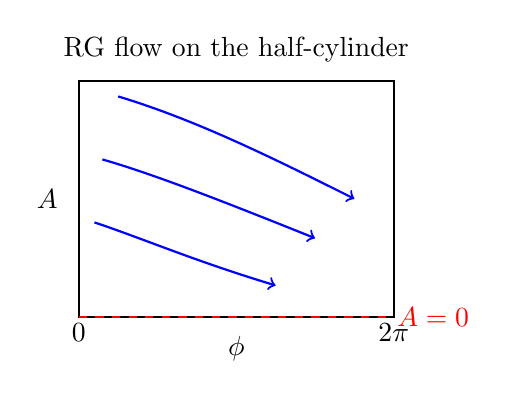
\begin{tikzpicture}[scale=1.0]
\draw[thick] (0,0) rectangle (4,3);
\node at (2,-0.4) {$\phi$};
\node at (-0.4,1.5) {$A$};
\node at (0,-0.2) {$0$};
\node at (4,-0.2) {$2\pi$};
\draw[thick, blue, ->] (0.5,2.8) .. controls (1.5,2.5) and (2.5,2.0) .. (3.5,1.5);
\draw[thick, blue, ->] (0.3,2.0) .. controls (1.0,1.8) and (2.0,1.4) .. (3.0,1.0);
\draw[thick, blue, ->] (0.2,1.2) .. controls (0.8,1.0) and (1.5,0.7) .. (2.5,0.4);
\draw[thick, red, dashed] (0,0) -- (4,0);
\node[red] at (4.5,0) {$A = 0$};
\node at (2,3.4) {RG flow on the half-cylinder};
\end{tikzpicture}
\end{center}

\subsection{The Fixed Point and Stability}

Setting $\boldsymbol{\beta} = 0$: $A^* = 0$ (oscillator at rest). This is a \textbf{stable} fixed point---all trajectories flow toward it.

\textbf{No anomalous dimension}: The oscillator has $\gamma = 0$ because energy conservation fixes the amplitude exactly. This contrasts with the PME and $\phi^4$ examples.

%-------------------------------------------------------------------------------
\section{Example 2: The Amplitude Equation}
\label{sec:amplitude_example}
%-------------------------------------------------------------------------------

\marginnote{The amplitude equation adds \textbf{nontrivial fixed points} to our toolkit---zeros of $\boldsymbol{\beta}$ beyond the trivial $A=0$.}

The oscillator (Section~\ref{sec:oscillator_example}) has only a trivial fixed point at $A = 0$. To see the full richness of RG flows~\eqref{eq:rg_ode}---including nontrivial fixed points where $\boldsymbol{\beta} = 0$ at nonzero coupling---we study the \textbf{amplitude equation}. This is the ``hydrogen atom'' of RG: analytically tractable with nontrivial structure.

\subsection{Physical Motivation}

Near a \textbf{Hopf bifurcation} or \textbf{pitchfork bifurcation}, many systems reduce to:
\begin{equation}
\boxed{\frac{dA}{dt} = \mu A - g|A|^2 A}
\label{eq:amplitude_equation}
\end{equation}
where $A$ is an amplitude, $\mu$ is the control parameter, and $g > 0$ is a saturation coefficient.

Examples include: laser physics ($A$ = field amplitude), fluid convection (Rayleigh-Bénard), and phase transitions ($A$ = order parameter).

\subsection{Fixed Points}

For real $A$, setting $\beta_A = 0$:
\begin{equation}
A(\mu - gA^2) = 0
\end{equation}

\textbf{Two fixed points:}
\begin{align}
A^*_{\text{trivial}} &= 0 \quad \text{(always exists)} \\
A^*_{\text{nontrivial}} &= \pm\sqrt{\frac{\mu}{g}} \quad \text{(exists only for } \mu > 0\text{)}
\end{align}

\begin{center}
\renewcommand{\arraystretch}{1.3}
\begin{tabular}{lcc}
\toprule
& \textbf{Amplitude Equation} & \textbf{$\phi^4$ Theory} \\
\midrule
Control parameter & $\mu$ & $\epsilon = 4 - d$ \\
Trivial fixed point & $A^* = 0$ & $\lambda^* = 0$ (Gaussian) \\
Nontrivial fixed point & $|A^*|^2 = \mu/g$ & $\lambda^* = 16\pi^2\epsilon/3$ (Wilson-Fisher) \\
Appearance condition & $\mu > 0$ & $\epsilon > 0$ (i.e., $d < 4$) \\
\bottomrule
\end{tabular}
\end{center}

\subsection{Exact Stability Analysis}

Linearize around each fixed point: $A = A^* + \delta A$.

\textbf{At $A^* = 0$:}
\begin{equation}
\left.\frac{d\beta_A}{dA}\right|_0 = \mu
\end{equation}
For $\mu < 0$: stable. For $\mu > 0$: unstable.

\textbf{At $|A^*|^2 = \mu/g$ (for $\mu > 0$):}
\begin{equation}
\left.\frac{d\beta_A}{dA}\right|_{A^*} = \mu - 3g|A^*|^2 = -2\mu
\end{equation}
The nontrivial fixed point is \textbf{stable} for $\mu > 0$.

\textbf{The bifurcation:} At $\mu = 0$, the two fixed points collide and exchange stability---a \textbf{supercritical pitchfork bifurcation}.

\subsection{Exact Solution}

The ODE solves exactly:
\begin{equation}
A(t) = \frac{A_0 \, e^{\mu t}}{\sqrt{1 + \frac{g A_0^2}{\mu}(e^{2\mu t} - 1)}}
\end{equation}

For $\mu > 0$: $A(t) \to \pm\sqrt{\mu/g}$ as $t \to \infty$. The system flows to the nontrivial fixed point.

\textbf{Key insight:} The amplitude equation captures the universal structure of RG near a bifurcation without requiring any loop calculations or $\epsilon$-expansion.

%-------------------------------------------------------------------------------
\section{Example 3: The Porous Medium Equation}
\label{sec:pme_example}
%-------------------------------------------------------------------------------

\marginnote{The PME introduces \textbf{anomalous dimensions}---the connection $\gamma$ from Section~\ref{sec:connections} becomes nontrivial.}

The oscillator and amplitude equation have $\gamma = 0$---no anomalous dimensions. The porous medium equation (PME) is our first example where the anomalous dimension (the connection coefficient from Section~\ref{sec:connections}) is \emph{nonzero}. Scaling exponents differ from dimensional analysis predictions because the nonlinearity ``renormalizes'' them.

\subsection{The Physical System}

The PME describes density evolution:
\begin{equation}
\frac{\partial\rho}{\partial t} = D\nabla^2(\rho^m)
\end{equation}
where $m > 0$ is the nonlinearity parameter. For $m = 1$, this is ordinary diffusion. For $m > 1$, diffusion is faster in high-density regions.

\subsection{Self-Similar Solutions}

Seek solutions of the form:
\begin{equation}
\rho(x,t) = t^{-\alpha}F(\xi), \qquad \xi = \frac{x}{t^\beta}
\end{equation}

Two constraints determine $(\alpha, \beta)$:

\textbf{Mass conservation:} $\alpha = d\beta$ (in $d$ dimensions)

\textbf{PME scaling:} $(m-1)\alpha = 2\beta - 1$

Solving:
\begin{equation}
\boxed{\beta = \frac{1}{2 + d(m-1)}, \qquad \alpha = \frac{d}{2 + d(m-1)}}
\end{equation}

\subsection{The Anomalous Dimension}

For linear diffusion ($m = 1$): $\beta = 1/2$ from dimensional analysis.

For $m \neq 1$, define the \textbf{anomalous dimension}:
\begin{equation}
\gamma_{\text{PME}} = \beta - \frac{1}{2} = -\frac{d(m-1)}{2(2 + d(m-1))}
\end{equation}

For $d = 1$, $m = 2$: $\gamma = -1/6$, so $\beta = 1/3$ instead of $1/2$.

\textbf{Physical interpretation:} The nonlinearity modifies the scaling behavior. The anomalous dimension quantifies how interactions change scaling---exactly as in QFT, where loop corrections modify classical dimensions.

\subsection{The Barenblatt Solution as Fixed Point}

The \textbf{Barenblatt solution}:
\begin{equation}
\rho(x,t) = t^{-\alpha}\left(C - \frac{m-1}{2m}\cdot\frac{\beta\xi^2}{D}\right)_+^{1/(m-1)}
\end{equation}
has compact support and is the \textbf{RG fixed point}---all reasonable initial conditions flow to it.

\begin{workedbox}[Box 2.5: Scaling Convention Independence in the PME]
\textbf{Goal:} Show that the PME exhibits the same invariance structure as QFT.

\textbf{The ``scaling convention'' for PME:} The similarity variable is $\xi = x/t^\beta$. Different choices of $\beta$ correspond to different \textbf{scaling conventions}---the PME analog of renormalization scheme choices. (We use ``scaling convention'' rather than ``scheme'' to avoid confusion with the QFT usage.)

\textbf{Scheme change:} Under $\beta \to \beta'$:
\begin{equation}
\xi' = x/t^{\beta'} = \xi \cdot t^{\beta - \beta'}
\end{equation}

\textbf{Physical invariants:}
\begin{itemize}
\item Total mass: $M = \int \rho\,dx$
\item Spreading rate: $L(t) \sim t^\alpha$ has the same exponent in all schemes
\item Shape near boundary
\end{itemize}

\tcblower
\textbf{The constraint algebra:} Not all choices of $\beta$ are valid. Mass conservation plus the PME give:
\begin{equation}
\alpha = d\beta, \qquad (m-1)\alpha = 2\beta - 1
\end{equation}

This restricts to a one-dimensional subspace of valid schemes. The physical exponent $\beta^* = 1/(d(m-1)+2)$ is the unique fixed point of this constraint algebra.
\end{workedbox}

%-------------------------------------------------------------------------------
\section{Example 4: The 1D $\phi^4$ Theory}
\label{sec:phi4_example}
%-------------------------------------------------------------------------------

\marginnote{$\phi^4$ theory exhibits all features: nontrivial fixed points, anomalous dimensions, operator mixing (Section~\ref{sec:connections}), and scheme dependence~\eqref{eq:beta_transform}.}

The previous examples were exactly solvable. $\phi^4$ theory requires perturbation theory, introducing loop corrections, operator mixing (the connection from Section~\ref{sec:connections}), and scheme dependence~\eqref{eq:beta_transform}. This example exercises the full framework: the CS equation~\eqref{eq:cs_full}, scheme transformations, and the bundle structure of Part~IV.

\subsection{The Setup}

The 1D $\phi^4$ theory has action:
\begin{equation}
S[\phi] = \int_0^L dx \left[ \frac{1}{2}\left(\frac{d\phi}{dx}\right)^2 + \frac{r}{2}\phi^2 + \frac{\lambda}{4}\phi^4 \right]
\end{equation}
with parameter space $\mathcal{M}_{\phi^4} = \{(r, \lambda) : \lambda > 0\}$.

\subsection{Wilson's Momentum-Shell RG}

\begin{workedbox}[Box 2.6: Momentum-Shell RG for 1D $\phi^4$ (Schematic)]
\textbf{Problem:} Derive beta functions using Wilson's procedure.

\textbf{Approximations:} This calculation is \textbf{schematic}---we work to leading order in $\lambda$ near the Gaussian fixed point. The propagator variance is approximate.

\textbf{Step 1: Field splitting.}
Write $\phi = \phi^< + \phi^>$ where $\phi^<$ has $|k| < \Lambda/b$ and $\phi^>$ has $\Lambda/b < |k| < \Lambda$.

\textbf{Step 2: Integrate out fast modes.}

For an infinitesimal shell $b = 1 + d\ell$:
\begin{equation}
\langle\phi^>(x)\phi^>(x)\rangle_0 \approx \frac{\Lambda}{\pi(\Lambda^2 + r)}d\ell
\end{equation}

This generates $\delta r = \frac{3\lambda\Lambda}{\pi(\Lambda^2 + r)}d\ell$.

\textbf{Step 3: Rescaling.}

Rescaling $x \to x/b$ gives:
\begin{equation}
r \to b^2 r, \qquad \lambda \to b^2\lambda
\end{equation}

\tcblower
\textbf{Result:}
\begin{equation}
\boxed{\beta_r = 2r + \frac{3\lambda\Lambda}{\pi(\Lambda^2 + r)}, \qquad \beta_\lambda = 2\lambda}
\end{equation}
\end{workedbox}

\subsection{The Full CS Equation}

For the two-point function:
\begin{equation}
\left(\Lambda\frac{\partial}{\partial\Lambda} + \beta_r\frac{\partial}{\partial r} + \beta_\lambda\frac{\partial}{\partial\lambda} + 2\gamma\right)\tilde{G}_2 = 0
\end{equation}

In 1D at one loop, $\gamma = 0$---the field has no anomalous dimension. This changes in higher dimensions!

\subsection{Operator Mixing}

The operators $\phi^2$ and $\phi^4$ mix under RG. The anomalous dimension matrix:
\begin{equation}
\gamma = \begin{pmatrix} \gamma_{\phi^2} & \gamma_{\phi^2\leftarrow\phi^4} \\ 0 & \gamma_{\phi^4} \end{pmatrix}
\end{equation}

The off-diagonal entry arises from tadpole diagrams: when we insert $\phi^4$, contracting two legs produces $\phi^2$.

\subsection{Preview: The Wilson-Fisher Fixed Point}

In $d = 4 - \epsilon$ dimensions, the one-loop beta function becomes:
\begin{equation}
\beta_\lambda = -\epsilon\lambda + \frac{3\lambda^2}{16\pi^2}
\end{equation}

Two fixed points:
\begin{itemize}
\item \textbf{Gaussian}: $\lambda^* = 0$ (free field theory)
\item \textbf{Wilson-Fisher}: $\lambda^*_{\text{WF}} = \frac{16\pi^2\epsilon}{3}$ (interacting)
\end{itemize}

The Wilson-Fisher fixed point exists for $d < 4$ and controls universal critical behavior near phase transitions.

\begin{workedbox}[Box 2.7: Dimensional Regularization and the $\overline{\text{MS}}$ Scheme]
\textbf{The problem:} Loop integrals in $d > 1$ are often UV divergent.

\textbf{Dimensional regularization:} Compute in $d = 4 - \epsilon$ and expand in $\epsilon$.

\textbf{Example: One-loop self-energy.}

The tadpole integral:
\begin{equation}
\Sigma = \frac{\lambda}{2}\int\frac{d^d k}{(2\pi)^d}\frac{1}{k^2 + m^2}
\end{equation}

In $d = 4 - \epsilon$, this has a $1/\epsilon$ pole.

\textbf{The $\overline{\text{MS}}$ scheme:} Subtract only the pole (and associated $\gamma_E - \log 4\pi$).

\tcblower
\textbf{The beta function emerges:}

Requiring $d\lambda_{\text{bare}}/d\mu = 0$:
\begin{equation}
\beta_\lambda = \mu\frac{d\lambda_R}{d\mu} = \frac{3\lambda^2}{16\pi^2} + O(\lambda^3) \quad \text{(in $d=4$)}
\end{equation}

\textbf{Key point:} The beta function is \textbf{scheme-independent} at leading order, but higher-order coefficients depend on the subtraction scheme.
\end{workedbox}

\subsection{Comparison of Examples}

\begin{center}
\renewcommand{\arraystretch}{1.3}
\begin{tabular}{lcccc}
\toprule
& \textbf{Oscillator} & \textbf{Amplitude} & \textbf{PME} & \textbf{$\phi^4$} \\
\midrule
Type & ODE & Normal form & PDE & Field theory \\
Scale $\ell$ & Time $t$ & Time $t$ & $\log t$ & Log-cutoff \\
Trivial FP & $A = 0$ & $A^* = 0$ & Dim.\ analysis & Gaussian \\
Nontrivial FP & --- & $|A^*|^2 = \mu/g$ & Barenblatt & Wilson-Fisher \\
Anomalous dim.? & No & No & Yes & Yes \\
Calculational & Exact & Exact & Self-similar & Perturbative \\
\bottomrule
\end{tabular}
\end{center}

%===============================================================================
% PART VI: ADVANCED GEOMETRIC TOPICS
%===============================================================================

\marginnote{Part VI develops additional geometric structures: curvature invariants, scheme independence as gauge invariance, and computational methods.}

Building on the metric from Section~\ref{sec:fisher_metric} and the connection from Section~\ref{sec:connections}, Part VI explores curvature invariants and computational methods.

%-------------------------------------------------------------------------------
\section{Curvature and Critical Exponents}
\label{sec:curvature_ch02}
%-------------------------------------------------------------------------------

\marginnote{The curvature of theory space encodes how operators respond to non-commuting deformations. It relates to universal data at fixed points.}

\subsection{The Curvature Tensor}

From the connection $\Gamma^a{}_{bc}$ introduced in Section~\ref{sec:connections}, we can compute the curvature tensor:
\begin{equation}
R^a{}_{bcd} = \partial_c\Gamma^a{}_{bd} - \partial_d\Gamma^a{}_{bc} + \Gamma^a{}_{ec}\Gamma^e{}_{bd} - \Gamma^a{}_{ed}\Gamma^e{}_{bc}
\label{eq:curvature_tensor}
\end{equation}

\textbf{Physical meaning:} Consider two deformations of a theory. If we first deform by $\delta g^c$ then $\delta g^d$, versus first $\delta g^d$ then $\delta g^c$, the curvature measures the difference:
\begin{equation}
[\nabla_c, \nabla_d]\mathcal{O}_a = R^b{}_{acd}\,\mathcal{O}_b
\end{equation}

The curvature tensor is a \textbf{tensor}---it transforms homogeneously under scheme changes. Curvature invariants (like $R^a{}_{bab}$, $R^a{}_{bcd}R^{bcd}{}_a$) are scheme-independent observables.

\subsection{Monodromy Around Singularities}

Even when the connection is flat (zero curvature), singularities can produce non-trivial \textbf{monodromy}. Parallel transporting around a singular point returns a transformed operator:
\begin{equation}
\mathcal{O}_a \to M^b{}_a\,\mathcal{O}_b, \qquad M = \exp\left(\oint \Gamma\,dg\right)
\end{equation}

This monodromy is closely related to \textbf{Stokes phenomena} in resurgent analysis.

\subsection{Curvature at Fixed Points}

At a fixed point, the curvature tensor contains universal data:
\begin{itemize}
\item \textbf{Eigenvalues} of the stability matrix (critical exponents)
\item \textbf{OPE coefficients} (structure constants of the CFT)
\item \textbf{Anomalous dimensions} of composite operators
\end{itemize}

Systems in the same universality class share these geometric invariants---this is the deep explanation of universality.

%-------------------------------------------------------------------------------
\section{Scheme Independence as Gauge Invariance}
\label{sec:scheme_gauge}
%-------------------------------------------------------------------------------

\marginnote{Scheme independence is mathematically identical to gauge invariance: the anomalous dimension transforms like a connection.}

The transformation~\eqref{eq:gamma_gauge_transform} of the anomalous dimension under scheme changes is precisely the gauge transformation law for a connection:
\begin{equation}
\gamma'_a{}^b = U_a{}^c\gamma_c{}^d(U^{-1})_d{}^b + \mu\frac{dU_a{}^c}{d\mu}(U^{-1})_c{}^b
\end{equation}

\textbf{Gauge-invariant quantities} (physical observables):
\begin{itemize}
\item Eigenvalues of $\gamma$ at fixed points (critical exponents)
\item Curvature invariants
\item Monodromy around closed loops in coupling space
\end{itemize}

\begin{workedbox}[Box 2.8: Covariant Expansion of Beta Functions]
\textbf{Goal:} Derive the metric from two-point functions following Dolan.

\textbf{Algebraic content:}

The metric arises from the \textbf{two-point function algebra}. For operators $\mathcal{O}_i$ and $\mathcal{O}_j$ conjugate to couplings $g^i$ and $g^j$:
\begin{equation}
G_{ij} = \int d^d x \, \langle \mathcal{O}_i(x) \mathcal{O}_j(0) \rangle_{\text{conn}}
\end{equation}

\textbf{Properties from unitarity:}
\begin{itemize}
\item \textbf{Symmetry}: $G_{ij} = G_{ji}$ (correlation functions are symmetric)
\item \textbf{Positivity}: $G_{ij}v^i v^j \geq 0$ for any $v$ (from reflection positivity)
\item \textbf{Grading}: $G_{ij} = 0$ if $\Delta_i \neq \Delta_j$ at a CFT fixed point
\end{itemize}

The positivity condition is an \textbf{algebraic constraint on representations}---it's the analog of requiring positive-definite norms in unitary representations.

\textbf{Geometric content:}

The metric $G_{ij}$ is a \textbf{Riemannian metric} on theory space. It measures ``distances'' between nearby theories:
\begin{equation}
ds^2 = G_{ij}(g) \, dg^i \, dg^j
\end{equation}

\textbf{QFT example: $\phi^4$ + Yukawa (Dolan):}

Consider a scalar $\phi$ with self-coupling $\lambda$ and Yukawa coupling $g$ to a fermion $\psi$:
\begin{equation}
\mathcal{L} = \frac{1}{2}(\partial\phi)^2 + \frac{\lambda}{4!}\phi^4 + \bar\psi(i\slashed\partial - m)\psi + g\phi\bar\psi\psi
\end{equation}

The metric components are:
\begin{align}
G_{\lambda\lambda} &= \frac{1}{576}\int d^d x \, \langle\phi^4(x)\phi^4(0)\rangle_{\text{conn}} \\
G_{\lambda g} &= \frac{1}{24}\int d^d x \, \langle\phi^4(x)(\bar\psi\psi\phi)(0)\rangle_{\text{conn}} \\
G_{gg} &= \int d^d x \, \langle(\bar\psi\psi\phi)(x)(\bar\psi\psi\phi)(0)\rangle_{\text{conn}}
\end{align}

\textbf{At one loop:}
\begin{equation}
G = \begin{pmatrix} A/\lambda^2 + O(1) & B/(\lambda g) + O(1) \\ B/(\lambda g) + O(1) & C/g^2 + O(1) \end{pmatrix}
\end{equation}
where $A$, $B$, $C$ are calculable from Feynman diagrams.

\tcblower
\textbf{Connection to central charge:} In 2D, the Zamolodchikov metric is related to the central charge via:
\begin{equation}
c \propto \text{tr}(G \cdot \gamma)
\end{equation}
where $\gamma$ is the anomalous dimension matrix. This is the origin of the c-theorem.
\end{workedbox}

\begin{workedbox}[Box 2.16: The Zamolodchikov Metric for the PME]
\textbf{Goal:} Construct the analog of the Zamolodchikov metric for the PME.

\textbf{The moment metric:}

For the PME, define the metric from \textbf{moment fluctuations}:
\begin{equation}
G_{mn} = \langle \delta M_m \, \delta M_n \rangle
\end{equation}
where $M_m = \int \xi^m F(\xi) \, d\xi$ are the moments of the self-similar profile.

\textbf{Connection to Fisher information:}

This is precisely the \textbf{Fisher information metric} for the family of Barenblatt profiles parameterized by $(m, d)$:
\begin{equation}
G_{ij}^{\text{(Fisher)}} = -\mathbb{E}\left[\frac{\partial^2 \log p(x|m,d)}{\partial g^i \partial g^j}\right]
\end{equation}
where $p(x|m,d) = F(\xi; m, d)$ is the profile interpreted as a probability distribution.

\textbf{Explicit calculation for $d = 1$:}

The Barenblatt profile is $F(\xi) = [C - k\xi^2]_+^{1/(m-1)}$. The Fisher metric has components:
\begin{equation}
G_{mm} \propto \int_{-\xi_0}^{\xi_0} \frac{1}{F}\left(\frac{\partial F}{\partial m}\right)^2 d\xi
\end{equation}

This integral diverges logarithmically as $m \to 1$ (approaching linear diffusion), reflecting the singular nature of the $m = 1$ limit.

\tcblower
\textbf{Geometric interpretation:}

The PME metric measures how ``distinguishable'' two Barenblatt profiles with different $m$ values are. Near $m = 1$, the profiles are infinitely distinguishable---the linear and nonlinear cases are ``infinitely far apart'' in metric terms.

This parallels the QFT situation: near a phase transition ($r \to r_c$), the susceptibility $\chi = G_{rr}$ diverges, making critical and non-critical theories infinitely distinguishable.
\end{workedbox}

\begin{workedbox}[Box 2.17: Sketch of the c-Theorem Proof]
\textbf{The c-function:} Define from stress tensor correlators:
\begin{equation}
c(r) = r^4\langle T(z)T(0)\rangle - \frac{3}{2}r^4\langle T(z)\Theta(0)\rangle - \frac{3}{16}r^4\langle\Theta(z)\Theta(0)\rangle
\end{equation}
where $T = T_{zz}$ is the holomorphic stress tensor and $\Theta = T_z{}^z$ is the trace.

\textbf{Conservation:} Stress tensor conservation $\partial_{\bar{z}}T = \partial_z\Theta$ implies:
\begin{equation}
r\frac{dc}{dr} = -\frac{3}{2}G(r), \quad G(r) = r^4\langle\Theta(z)\Theta(0)\rangle
\end{equation}

\textbf{Unitarity:} In a unitary theory, $G(r) \geq 0$ because $\Theta$ is Hermitian.

\tcblower
\textbf{Conclusion:} Since $r \sim e^{-\ell}$, we have $\frac{dc}{d\ell} = -r\frac{dc}{dr} = \frac{3}{2}G \geq 0$... 

Wait, this gives $dc/d\ell \geq 0$, the opposite sign! The resolution is that increasing $\ell$ means flowing to the IR (lower energy), and $c$ \textit{decreases} in the IR direction:
\begin{equation}
\boxed{\frac{dc}{d\ell} \leq 0 \quad \text{(flowing toward IR)}}
\end{equation}
\end{workedbox}

\begin{workedbox}[Box 2.18: Potential Flow and Integrability (Dolan)]
\textbf{Goal:} Verify that RG flow is potential flow in Dolan's $\phi^4$ + Yukawa model.

\textbf{Algebraic content:}

Potential flow means the beta function is a gradient:
\begin{equation}
\beta^i = G^{ij} \frac{\partial W}{\partial g^j}
\end{equation}
for some potential $W(g)$ and metric $G_{ij}$.

\textbf{The integrability condition:}

Lowering the index: $\beta_i = G_{ij}\beta^j$. Potential flow requires $\beta_i = \partial_i W$, which implies:
\begin{equation}
\partial_i \beta_j = \partial_j \beta_i \quad \text{(symmetry of mixed partials)}
\end{equation}

This is the \textbf{integrability condition}---an algebraic constraint that must be checked order by order.

\textbf{In algebraic terms:} The integrability condition is a \textbf{cocycle condition} in the de Rham complex:
\begin{equation}
d\beta^\flat = 0 \quad \Leftrightarrow \quad \beta^\flat = dW
\end{equation}
where $\beta^\flat = G_{ij}\beta^j dg^i$ is the 1-form associated to $\beta$.

\textbf{Dolan's verification (to sixth order):}

For the $\phi^4$ + Yukawa model with couplings $(\lambda, g)$, Dolan computed:
\begin{align}
\beta_\lambda &= -\epsilon\lambda + a_1\lambda^2 + a_2 g^2\lambda + a_3\lambda^3 + \cdots \\
\beta_g &= -\frac{\epsilon}{2}g + b_1 g\lambda + b_2 g^3 + b_3 g\lambda^2 + \cdots
\end{align}

The integrability condition $\partial_\lambda\beta_g = \partial_g\beta_\lambda$ gives:
\begin{equation}
b_1 + \text{(corrections)} = 2a_2 + \text{(corrections)}
\end{equation}

\textbf{Result:} Dolan verified this to sixth order in the couplings. The RG flow \textbf{is} potential flow, at least perturbatively.

\tcblower
\textbf{The c-function as Casimir:}

When integrability holds, the potential $W$ is the c-function:
\begin{equation}
\frac{dW}{d\ell} = \beta^i \partial_i W = \beta^i G_{ij} \beta^j = G_{ij}\beta^i\beta^j \geq 0
\end{equation}

The c-function is a \textbf{Casimir invariant} of the flow: it labels orbits and increases monotonically.
\end{workedbox}

\begin{workedbox}[Box 2.19: Potential Flow in the PME]
\textbf{Goal:} Show the PME has gradient flow structure.

\textbf{The Lyapunov functional:}

The PME admits a Lyapunov functional:
\begin{equation}
\mathcal{F}[\rho] = \int \left[\frac{1}{m}\rho^m + \frac{1}{2}V(x)\rho\right] d^d x
\end{equation}
(for PME with external potential $V$; for free PME, take $V = 0$).

\textbf{Gradient flow structure:}

The PME can be written as:
\begin{equation}
\partial_t \rho = \nabla \cdot \left(\rho \nabla \frac{\delta\mathcal{F}}{\delta\rho}\right)
\end{equation}

This is gradient flow in the \textbf{Wasserstein metric}:
\begin{equation}
\partial_t \rho = -\text{grad}_W \mathcal{F}
\end{equation}
where $\text{grad}_W$ is the gradient with respect to the Wasserstein-2 distance.

\textbf{Entropy production:}

Along the flow:
\begin{equation}
\frac{d\mathcal{F}}{dt} = -\int \rho \left|\nabla\frac{\delta\mathcal{F}}{\delta\rho}\right|^2 d^d x \leq 0
\end{equation}

This is the PME analog of the c-theorem: entropy decreases monotonically.

\tcblower
\textbf{Message:} Both QFT and the PME exhibit gradient flow structure. This is why c-theorem-type results hold: the RG ``potential'' (c-function or entropy) must decrease.
\end{workedbox}

%-------------------------------------------------------------------------------
\section{Solving RG Equations}
\label{sec:solving_rg}
%-------------------------------------------------------------------------------

\marginnote{The CS equation~\eqref{eq:callan_symanzik_basic} is a first-order PDE. Solving it gives the scale dependence of observables.}

The CS equation~\eqref{eq:callan_symanzik_basic} is a first-order PDE. The method of characteristics solves it.

\subsection{The Method of Characteristics}

The equation:
\begin{equation}
\left(\mu\frac{\partial}{\partial\mu} + \beta(g)\frac{\partial}{\partial g}\right)\mathcal{O} = 0
\end{equation}
says $\mathcal{O}$ is constant along characteristic curves. The characteristics are the RG trajectories~\eqref{eq:rg_ode}:
\begin{equation}
\mu\frac{dg}{d\mu} = \beta(g)
\end{equation}

The \textbf{running coupling} $\bar{g}(\mu; g_0, \mu_0)$ solves this with initial condition $\bar{g}(\mu_0) = g_0$.

\begin{workedbox}[Box 2.9: Running Couplings for 1D $\phi^4$]
\textbf{Goal:} Solve the RG equations for $r(\ell)$ and $\lambda(\ell)$.

\textbf{The equations:}
\begin{align}
\frac{dr}{d\ell} &= 2r + \frac{3\lambda\Lambda}{\pi(\Lambda^2 + r)} \\
\frac{d\lambda}{d\ell} &= 2\lambda
\end{align}

\textbf{Solution for $\lambda$:}
\begin{equation}
\lambda(\ell) = \lambda_0 e^{2\ell}
\end{equation}

\textbf{Solution for $r$ (near Gaussian):}
\begin{equation}
r(\ell) = \left(r_0 + \frac{3\lambda_0\ell}{\pi\Lambda}\right)e^{2\ell}
\end{equation}

\tcblower
\textbf{Physical interpretation:}
\begin{itemize}
\item Both $r$ and $\lambda$ grow as we zoom out
\item Even if $r_0 = 0$, fluctuations generate $r > 0$: the tadpole ``dresses'' the mass
\item The Gaussian fixed point is unstable in both directions
\end{itemize}
\end{workedbox}

\subsection{RG-Improved Correlation Functions}

With running couplings, physical predictions are independent of which scale we use:
\begin{equation}
\tilde{G}_2(p; r_0, \lambda_0, \Lambda_0) = \tilde{G}_2(p; r(\Lambda), \lambda(\Lambda), \Lambda)
\end{equation}

%-------------------------------------------------------------------------------
\section{Asymptotic Behavior and the Landau Pole}
\label{sec:asymptotic}
%-------------------------------------------------------------------------------

\marginnote{Classification of theories by asymptotic behavior: asymptotic freedom vs infrared freedom.}

\subsection{Classification of Theories}

\textbf{Asymptotic freedom} ($\beta < 0$ for small $g$): Coupling decreases in UV. QCD is the canonical example.

\textbf{Infrared freedom} ($\beta > 0$ for small $g$): Coupling decreases in IR. This is 1D $\phi^4$.

\subsection{The Landau Pole}

When $\beta > 0$, the running coupling can diverge at finite scale. For $\beta = bg^2$:
\begin{equation}
g(\mu) = \frac{g_0}{1 - bg_0\log(\mu/\mu_0)}
\end{equation}

This diverges at $\mu_{\text{Landau}} = \mu_0 \exp(1/(bg_0))$---the \textbf{Landau pole}.

\subsection{The RG as a Semigroup}

\marginnote{A semigroup has closure and associativity but lacks inverses. The RG can fail to be invertible.}

The RG can fail to be a group for two reasons:
\begin{enumerate}
\item \textbf{Information loss (coarse-graining):} Wilson's RG integrates out degrees of freedom. Once averaged away, information cannot be recovered.
\item \textbf{Perturbative singularities:} The Landau pole means the flow is only defined on a restricted domain.
\end{enumerate}

%-------------------------------------------------------------------------------
\section{From Perturbative to Exact: The Functional RG}
\label{sec:exact_rg}
%-------------------------------------------------------------------------------

\marginnote{The exact RG provides a functional differential equation whose perturbative expansion recovers the CS equation.}

The perturbative RG is powerful but limited. The \textbf{Exact Renormalization Group} (ERG) treats the RG exactly.

\subsection{The Polchinski Equation}

Wilson's insight: the RG is an exact transformation on the space of \textit{actions}. The Polchinski equation describes how the effective action $S_\Lambda[\phi]$ changes as we lower the cutoff:
\begin{equation}
\Lambda\frac{\partial S_\Lambda}{\partial\Lambda} = \frac{1}{2}\int\frac{d^dp}{(2\pi)^d}\,\dot{K}\left[\frac{\delta S}{\delta\phi(p)}\frac{\delta S}{\delta\phi(-p)} - \frac{\delta^2 S}{\delta\phi(p)\delta\phi(-p)}\right]
\end{equation}

This is \textit{exact}---no perturbation theory invoked.

\subsection{The Derivative Expansion}

Expand $S_\Lambda$ in derivatives:
\begin{equation}
S_\Lambda[\phi] = \int d^dx\left[V_\Lambda(\phi) + \frac{1}{2}Z_\Lambda(\phi)(\partial\phi)^2 + O(\partial^4)\right]
\end{equation}

The \textbf{Local Potential Approximation (LPA)} keeps only $V_\Lambda(\phi)$. This gives a tractable PDE for finding fixed points non-perturbatively.

%-------------------------------------------------------------------------------
\section{Looking Ahead}
\label{sec:looking_ahead}
%-------------------------------------------------------------------------------

This chapter established the complete RG framework, showing that \textbf{algebra and geometry are two faces of the same structure}:

\textbf{The central equation:} The Callan-Symanzik equation~\eqref{eq:callan_symanzik_basic} encodes scale independence

\textbf{Symmetry structure (Part II):} Scale invariance gives a Lie group (Section~\ref{sec:dilation_algebra}); scheme invariance gives diffeomorphisms (Section~\ref{sec:scheme_algebra})

\textbf{Geometric realization (Part III):} These symmetries are naturally geometric---parameter space is a manifold, $\beta$~\eqref{eq:beta_vector_field} is a vector field, $\gamma$ is a connection, and the Fisher metric completes the picture

\textbf{Unified picture (Part IV):} The gauge bundle structure unifies diffeomorphisms and gauge transformations (Section~\ref{sec:gauge_bundle})

\textbf{Examples (Part V):} Four examples of increasing complexity demonstrate the unified framework

\textbf{Advanced topics (Part VI):} Curvature invariants, solving RG equations, and the exact RG

\marginnote{Chapter~\ref{ch:fixed_points} focuses on the zeros of $\boldsymbol{\beta}$: fixed points, universality, and scaling.}

Chapter~\ref{ch:fixed_points} focuses on the zeros of $\boldsymbol{\beta}$---the fixed points:
\begin{itemize}
\item Fixed-point classification and stability (eigenvalues of $\partial_j\beta^i|_{g^*}$)
\item Critical exponents and universality classes
\item Normal form theory for RG flows
\item The role of marginal operators and logarithmic corrections
\end{itemize}

Part II then turns to \textbf{analytical methods}: perturbation theory (with its asymptotic series) and transseries (capturing non-perturbative physics).

%-------------------------------------------------------------------------------
\section*{Exercises}
\addcontentsline{toc}{section}{Exercises}
%-------------------------------------------------------------------------------

\begin{enumerate}
\item \textbf{The dilation Lie algebra.} Verify that $\mathcal{D} = x^\mu\partial_\mu$ generates scale transformations: $e^{\ell\mathcal{D}}f(x) = f(e^\ell x)$.

\item \textbf{Dilation as a group action.} Consider $D_\lambda: f(x) \mapsto f(\lambda x)$.
\begin{enumerate}
\item Show that $D_\lambda D_\mu = D_{\lambda\mu}$.
\item For homogeneous functions $f(\lambda x) = \lambda^\Delta f(x)$, show that $\Delta$ is the eigenvalue of $x\frac{d}{dx}$.
\end{enumerate}

\item \textbf{RG as Lie transport.} For $\boldsymbol{\beta} = -\gamma A\partial_A + \frac{3\epsilon A^2}{8\omega_0}\partial_\phi$:
\begin{enumerate}
\item Compute $e^{t\boldsymbol{\beta}}$ acting on $(A, \phi)$.
\item Show any function $f(A)$ has $L_{\boldsymbol{\beta}}f = -\gamma A\frac{\partial f}{\partial A}$.
\end{enumerate}

\item \textbf{CS equation verification.} For the 1D $\phi^4$ four-point function $G_4$ at tree level:
\begin{enumerate}
\item Write $G_4$ in terms of $\lambda$ and propagators.
\item Verify $(\Lambda\partial_\Lambda + \beta_r\partial_r + \beta_\lambda\partial_\lambda + 4\gamma)G_4 = 0$ with $\gamma = 0$.
\end{enumerate}

\item \textbf{Running mass.} Solve the RG equations for $r(\ell)$ including the tadpole.
\begin{enumerate}
\item Show that even if $r_0 = 0$, a mass is generated.
\item Find the ``critical'' $r_0$ for which $r(\ell) \to 0$ as $\ell \to \infty$.
\end{enumerate}

\item \textbf{Landau pole in QED.} The beta function is $\beta_\alpha = \frac{2\alpha^2}{3\pi}$.
\begin{enumerate}
\item Solve for $\alpha(\mu)$.
\item Find $\mu_{\text{Landau}}$ in terms of $\alpha_0$ and $\mu_0$.
\item Estimate numerically using $\alpha(m_e) \approx 1/137$.
\end{enumerate}

\item \textbf{Wilson-Fisher fixed point.} For $\beta_\lambda = -\epsilon\lambda + 3\lambda^2/(16\pi^2)$:
\begin{enumerate}
\item Find the fixed points $\lambda^*$.
\item Identify UV-attractive vs IR-attractive.
\item Solve for $\lambda(\mu)$ interpolating between them.
\end{enumerate}

\item \textbf{The van der Pol oscillator.} For $\ddot{x} - \epsilon(1-x^2)\dot{x} + x = 0$:
\begin{enumerate}
\item Use multiple scales with $\tau = \epsilon t$.
\item Show $dA/d\tau = A(1 - A^2/4)/2$.
\item Find the fixed point and interpret physically.
\end{enumerate}

\item \textbf{Gevrey-1 structure.} For $\tilde{f}(\epsilon) = \sum_{n=0}^\infty (-1)^n n! \epsilon^{n+1}$:
\begin{enumerate}
\item Verify Gevrey-1: $|a_n| \leq C \cdot K^n \cdot n!$.
\item Compute the Borel transform $\hat{f}_B(\zeta)$.
\item Identify the singularity and explain the alternating signs.
\end{enumerate}
\end{enumerate}

%-------------------------------------------------------------------------------
\section*{Summary}
\addcontentsline{toc}{section}{Summary}
%-------------------------------------------------------------------------------

\begin{summarybox}

\summaryheader{The Central Equation}
The Callan-Symanzik equation~\eqref{eq:callan_symanzik_basic} encodes scale independence:
\begin{equation}
\left(\mu\frac{\partial}{\partial\mu} + \beta^i(g)\frac{\partial}{\partial g^i} + n\gamma(g)\right)G_n = 0
\tag{\ref{eq:cs_full}}
\end{equation}

\summaryheader{Symmetry Structure (Part II)}
\begin{itemize}
\item \textbf{Scale invariance}: gives the dilation Lie group with generator~\eqref{eq:dilation_generator}
\item \textbf{Scheme invariance}: beta transforms as~\eqref{eq:beta_transform}---this IS the vector field law
\item \textbf{Scaling dimensions}: eigenvalues~\eqref{eq:scaling_eigenvalue} of the generator
\end{itemize}

\summaryheader{Geometric Realization (Part III)}
The symmetry structure IS geometric:
\begin{itemize}
\item Couplings $g^i$ are coordinates on manifold $\mathcal{M}$; schemes are coordinates
\item Beta function~\eqref{eq:beta_vector_field} is a vector field; flows~\eqref{eq:rg_ode} are integral curves
\item Anomalous dimension $\gamma_a{}^b$ is a connection
\item Fisher metric $G_{ab}$~\eqref{eq:fisher_metric} measures distances
\item Gradient flow~\eqref{eq:gradient_flow_ansatz} and geodesics complete the picture
\end{itemize}

\summaryheader{Unified Picture (Part IV)}
Theory space is a \textbf{gauge bundle}. Scheme changes are diffeomorphisms on base + gauge on fiber.

\summaryheader{The Four Examples}
\begin{center}
\renewcommand{\arraystretch}{1.2}
\begin{tabular}{lcccc}
& \textbf{Oscillator} & \textbf{Amplitude} & \textbf{PME} & \textbf{$\phi^4$} \\
\hline
Nontrivial FP? & No & Yes & Yes & Yes \\
Anomalous dim? & No & No & Yes & Yes \\
\end{tabular}
\end{center}

\summaryheader{Key Insight}
Algebra and geometry are not alternative perspectives---they are two faces of the same structure emerging from~\eqref{eq:callan_symanzik_basic}.

\end{summarybox}

%-------------------------------------------------------------------------------
\section*{Exercises}
\addcontentsline{toc}{section}{Exercises}
%-------------------------------------------------------------------------------

\begin{enumerate}
\item \textbf{The dilation Lie algebra.} Verify that $\mathcal{D} = x^\mu\partial_\mu$, $P_\mu = \partial_\mu$, and $K_\mu = 2x_\mu x^\nu\partial_\nu - x^2\partial_\mu$ satisfy the conformal algebra commutation relations in $d$ dimensions.

\item \textbf{Dilation as a group action.} Consider $D_\lambda: f(x) \mapsto f(\lambda x)$.
\begin{enumerate}
\item Show that $D_\lambda D_\mu = D_{\lambda\mu}$.
\item For homogeneous functions $f(\lambda x) = \lambda^\Delta f(x)$, show that $\Delta$ is the eigenvalue of $x\frac{d}{dx}$.
\end{enumerate}

\item \textbf{RG as Lie transport.} For $\boldsymbol{\beta} = -\gamma A\partial_A + \frac{3\epsilon A^2}{8\omega_0}\partial_\phi$:
\begin{enumerate}
\item Compute $e^{t\boldsymbol{\beta}}$ acting on $(A, \phi)$.
\item Show any function $f(A)$ has $L_{\boldsymbol{\beta}}f = -\gamma A\frac{\partial f}{\partial A}$.
\end{enumerate}

\item \textbf{CS equation verification.} For the 1D $\phi^4$ four-point function $G_4$ at tree level:
\begin{enumerate}
\item Write $G_4$ in terms of $\lambda$ and propagators.
\item Verify $(\Lambda\partial_\Lambda + \beta_r\partial_r + \beta_\lambda\partial_\lambda + 4\gamma)G_4 = 0$ with $\gamma = 0$.
\end{enumerate}

\item \textbf{Running mass.} Solve the RG equations for $r(\ell)$ including the tadpole.
\begin{enumerate}
\item Show that even if $r_0 = 0$, a mass is generated.
\item Find the ``critical'' $r_0$ for which $r(\ell) \to 0$ as $\ell \to \infty$.
\end{enumerate}

\item \textbf{Landau pole in QED.} The beta function is $\beta_\alpha = \frac{2\alpha^2}{3\pi}$.
\begin{enumerate}
\item Solve for $\alpha(\mu)$.
\item Find $\mu_{\text{Landau}}$ in terms of $\alpha_0$ and $\mu_0$.
\item Estimate numerically using $\alpha(m_e) \approx 1/137$.
\end{enumerate}

\item \textbf{Wilson-Fisher fixed point.} For $\beta_\lambda = -\epsilon\lambda + 3\lambda^2/(16\pi^2)$:
\begin{enumerate}
\item Find the fixed points $\lambda^*$.
\item Identify UV-attractive vs IR-attractive.
\item Solve for $\lambda(\mu)$ interpolating between them.
\end{enumerate}

\item \textbf{The van der Pol oscillator.} For $\ddot{x} - \epsilon(1-x^2)\dot{x} + x = 0$:
\begin{enumerate}
\item Use multiple scales with $\tau = \epsilon t$.
\item Show $dA/d\tau = A(1 - A^2/4)/2$.
\item Find the fixed point and interpret physically.
\end{enumerate}

\item \textbf{Gevrey-1 structure.} For $\tilde{f}(\epsilon) = \sum_{n=0}^\infty (-1)^n n! \epsilon^{n+1}$:
\begin{enumerate}
\item Verify Gevrey-1: $|a_n| \leq C \cdot K^n \cdot n!$.
\item Compute the Borel transform $\hat{f}_B(\zeta)$.
\item Identify the singularity and explain the alternating signs.
\end{enumerate}
\end{enumerate}

%-------------------------------------------------------------------------------
\section*{Summary}
\addcontentsline{toc}{section}{Summary}
%-------------------------------------------------------------------------------

\begin{summarybox}

\summaryheader{The Central Equation}
The Callan-Symanzik equation~\eqref{eq:callan_symanzik_basic} encodes scale independence:
\begin{equation}
\left(\mu\frac{\partial}{\partial\mu} + \beta^i(g)\frac{\partial}{\partial g^i} + n\gamma(g)\right)G_n = 0
\tag{\ref{eq:cs_full}}
\end{equation}

\summaryheader{Symmetry Structure (Part II)}
\begin{itemize}
\item \textbf{Scale invariance}: gives the dilation Lie group with generator~\eqref{eq:dilation_generator}
\item \textbf{Scheme invariance}: beta transforms as~\eqref{eq:beta_transform}---this IS the vector field law
\item \textbf{Scaling dimensions}: eigenvalues~\eqref{eq:scaling_eigenvalue} of the generator
\end{itemize}

\summaryheader{Geometric Realization (Part III)}
The symmetry structure IS geometric:
\begin{itemize}
\item Couplings $g^i$ are coordinates on manifold $\mathcal{M}$; schemes are coordinates
\item Beta function~\eqref{eq:beta_vector_field} is a vector field; flows~\eqref{eq:rg_ode} are integral curves
\item Anomalous dimension $\gamma_a{}^b$ is a connection
\end{itemize}

\summaryheader{Unified Picture (Part IV)}
Theory space is a \textbf{gauge bundle}. Scheme changes are diffeomorphisms on base + gauge on fiber.

\summaryheader{Metric Structure (Part VI)}
The Fisher metric enables gradient flow~\eqref{eq:gradient_flow_ansatz} and geodesic interpretations.

\summaryheader{The Four Examples}
\begin{center}
\renewcommand{\arraystretch}{1.2}
\begin{tabular}{lcccc}
& \textbf{Oscillator} & \textbf{Amplitude} & \textbf{PME} & \textbf{$\phi^4$} \\
\hline
Nontrivial FP? & No & Yes & Yes & Yes \\
Anomalous dim? & No & No & Yes & Yes \\
\end{tabular}
\end{center}

\summaryheader{Key Insight}
Algebra and geometry are not alternative perspectives---they are two faces of the same structure emerging from~\eqref{eq:callan_symanzik_basic}.

\end{summarybox}

%-------------------------------------------------------------------------------
% EXERCISE SOLUTIONS
%-------------------------------------------------------------------------------

\begin{solutionbox}[Solution to Exercise 2.1: The dilation Lie algebra]
\textbf{Commutator $[\mathcal{D}, P_\mu]$:}

Acting on test function $f$:
\begin{align}
[\mathcal{D}, P_\mu]f &= x^\nu\partial_\nu(\partial_\mu f) - \partial_\mu(x^\nu\partial_\nu f) \\
&= x^\nu\partial_\nu\partial_\mu f - \delta_\mu^\nu\partial_\nu f - x^\nu\partial_\mu\partial_\nu f = -\partial_\mu f
\end{align}
Result: $\boxed{[\mathcal{D}, P_\mu] = -P_\mu}$

\textbf{Commutator $[\mathcal{D}, K_\mu]$:}

After computation: $[\mathcal{D}, K_\mu]f = K_\mu f$

Result: $\boxed{[\mathcal{D}, K_\mu] = K_\mu}$

\textbf{Commutator $[P_\mu, K_\nu]$:}

After computation: $[P_\mu, K_\nu]f = 2\eta_{\mu\nu}\mathcal{D}f - 2M_{\mu\nu}f$

Result: $\boxed{[P_\mu, K_\nu] = 2(\eta_{\mu\nu}\mathcal{D} - M_{\mu\nu})}$
\end{solutionbox}

\begin{solutionbox}[Solution to Exercise 2.2: Dilation as a group action]
\textbf{(a) Composition law.}

$(D_\lambda D_\mu)f(x) = D_\lambda[f(\mu x)] = f(\mu(\lambda x)) = f((\lambda\mu)x) = D_{\lambda\mu}f(x)$

Therefore: $\boxed{D_\lambda D_\mu = D_{\lambda\mu}}$

\textbf{(b) Homogeneous functions.}

Differentiate $f(\lambda x) = \lambda^\Delta f(x)$ w.r.t.\ $\lambda$ and set $\lambda = 1$:

$xf'(x) = \Delta f(x)$, i.e., $\boxed{\mathcal{D}f = \Delta f}$
\end{solutionbox}

\begin{solutionbox}[Solution to Exercise 2.3: RG as Lie transport]
\textbf{(a)} The flow equations give $A(t) = A_0 e^{-\gamma t}$ and $\phi(t) = \phi_0 + \frac{3\epsilon}{16\gamma\omega_0}A_0^2(1 - e^{-2\gamma t})$.

$\boxed{e^{t\boldsymbol{\beta}}(A_0, \phi_0) = \left(A_0 e^{-\gamma t}, \phi_0 + \frac{3\epsilon A_0^2}{16\gamma\omega_0}(1 - e^{-2\gamma t})\right)}$

\textbf{(b)} $L_{\boldsymbol{\beta}}f = -\gamma A\frac{\partial f}{\partial A} + \frac{3\epsilon A^2}{8\omega_0}\frac{\partial f}{\partial\phi} = -\gamma A\frac{\partial f}{\partial A}$ for $f = f(A)$.
\end{solutionbox}

\begin{solutionbox}[Solution to Exercise 2.5: Running mass]
\textbf{(a) Mass generation.}

With $r_0 = 0$: $r(\ell) = \frac{3\lambda_0}{\pi\Lambda_0}(e^{3\ell} - e^{2\ell})$

For large $\ell$: $\boxed{r(\ell) \approx \frac{3\lambda_0}{\pi\Lambda_0}e^{3\ell} > 0}$

A positive mass is generated by fluctuations!

\textbf{(b) Physical interpretation.}

In statistical mechanics, $r \propto (T - T_c)$. The generation of positive mass means fluctuations disorder the system---the Coleman-Mermin-Wagner phenomenon in 1D.
\end{solutionbox}

\begin{solutionbox}[Solution to Exercise 2.6: Landau pole in QED]
\textbf{(a)} Separating variables: $\boxed{\alpha(\mu) = \frac{\alpha_0}{1 - \frac{2\alpha_0}{3\pi}\ln(\mu/\mu_0)}}$

\textbf{(b)} Diverges when denominator vanishes: $\boxed{\mu_{\text{Landau}} = \mu_0\exp\left(\frac{3\pi}{2\alpha_0}\right)}$

\textbf{(c)} With $\alpha_0 = 1/137$ at $\mu_0 = m_e$:

$\frac{3\pi}{2\alpha_0} = \frac{3\pi \times 137}{2} \approx 645$

$\mu_{\text{Landau}} \approx m_e \cdot e^{645} \approx 10^{280}$ MeV $\approx 10^{277}$ GeV

Far beyond the Planck scale---considered unphysical.
\end{solutionbox}

\begin{solutionbox}[Solution to Exercise 2.7: Wilson-Fisher fixed point]
\textbf{(a) Fixed points.}

$\lambda(-\epsilon + \frac{3\lambda}{16\pi^2}) = 0$

$\lambda_1^* = 0$ (Gaussian), $\lambda_2^* = \frac{16\pi^2\epsilon}{3}$ (Wilson-Fisher)

\textbf{(b) Stability.}

At $\lambda = 0$: $\beta'(0) = -\epsilon < 0$ for $\epsilon > 0$ $\Rightarrow$ unstable (IR-repulsive)

At $\lambda^*_{\text{WF}}$: $\beta'(\lambda^*) = +\epsilon > 0$ $\Rightarrow$ stable (IR-attractive)

\textbf{(c) Solution.}

$\boxed{\lambda(\mu) = \frac{16\pi^2\epsilon/3}{1 + C(16\pi^2\epsilon/3)\mu^\epsilon}}$

As $\mu \to 0$: $\lambda \to \lambda^*_{\text{WF}}$. As $\mu \to \infty$: $\lambda \to 0$.
\end{solutionbox}

\begin{solutionbox}[Solution to Exercise 2.8: The van der Pol oscillator]
\textbf{(a)} Multiple scales with $\tau = \epsilon t$, $x_0 = A(\tau)\cos(t + \phi(\tau))$.

\textbf{(b)} Canceling secular terms:
$\boxed{\frac{dA}{d\tau} = \frac{A}{2}\left(1 - \frac{A^2}{4}\right)}$

\textbf{(c)} Fixed points: $A = 0$ (unstable) and $A = 2$ (stable).

Physical interpretation: The van der Pol oscillator has a \textbf{limit cycle} at $A = 2$. Small oscillations grow; large oscillations are damped. The system settles to a stable periodic orbit.
\end{solutionbox}

\begin{solutionbox}[Solution to Exercise 2.9: Gevrey-1 structure]
\textbf{(a)} For $n \geq 1$: $|a_n| = (n-1)! \leq n!$. With $C = 1$, $K = 1$: Gevrey-1. \checkmark

\textbf{(b)} $\hat{f}_B(\zeta) = \sum_{n=1}^\infty \frac{(-1)^{n-1}}{n}\zeta^n = \boxed{\log(1+\zeta)}$

\textbf{(c)} Branch point at $\zeta = -1$ (negative real axis).

Alternating signs mean the series is Borel-summable along the positive real axis. Singularity at $\zeta < 0$ corresponds to an ``anti-instanton.''
\end{solutionbox}

